%% Type de document et encodage de la police
\documentclass[a4paper]{article}
\usepackage[utf8x]{inputenc}
\usepackage[T1]{fontenc}

%% Initialise la taille des pages et des marges
\usepackage[a4paper, top=3cm, bottom=3cm, left=2cm, right=2cm, marginparwidth=2cm]{geometry}

%% Commandes perso
\renewcommand{\arraystretch}{1.2} %% row 20% longer
\renewcommand{\contentsname}{Table des matières}

%% Pour les exemples
\usepackage{mdframed}
\newmdenv[topline=false, bottomline=false, rightline=false, skipabove=\topsep, skipbelow=\topsep]{example}

%% Pour les diagrammes
\usepackage{tikz}
\usepackage[american,cuteinductors,smartlabels]{circuitikz}
\usetikzlibrary{calc}
\tikzstyle{incolore} = [rectangle, rounded corners, draw=black, minimum height=1cm, minimum width=3cm, text width=3cm, text centered]
\tikzstyle{rect} = [rectangle, draw=black, minimum height=1cm, minimum width=3cm, text centered, anchor=north west]

%% Packs utiles
\usepackage{amsmath}
\usepackage{graphicx}
\usepackage[colorlinks=true, allcolors=black]{hyperref}

%% Pour le code
\usepackage{listings}
\lstdefinestyle{customc}{
    belowcaptionskip=1\baselineskip,
    breaklines=true,
    frame=L,
    xleftmargin=\parindent,
    language=C,
    showstringspaces=false,
    basicstyle=\footnotesize\ttfamily,
    keywordstyle=\bfseries\color{green!40!black},
    commentstyle=\itshape\color{purple!40!black},
    identifierstyle=\color{blue},
    stringstyle=\color{orange},
    numbers=left,
    stepnumber=1,
}
\lstset{escapechar=@,style=customc}
%\lstset{language=C++}


\title{Systèmes Embarqués Examen 2019}
\author{Grégoire Roumache}
\date{Avril 2020}

\begin{document}

\maketitle




















\part{Théorie \& Exercices}















\section{Rappel théorique}










\subsection{Rappel général}





\begin{itemize}


\item TIC = Tension inverse maximale = tension maximale que la diode peut prendre en sens inverse avant de claquer.


\item Caractéristiques du réseau électrique en Belgique:
\begin{itemize}
    \item $ f = 50 \; [Hz] $
    \item $ U_{max} = 230 \; [V] $
\end{itemize}


\item coefficient d'ondulation = $\displaystyle \frac{\text{tension efficace}}{\text{tension moyenne}} $


\item Tableau récapitulatif:
\begin{center}
    \begin{tabular}{c|c|c|c|c}
        & $ f $ & $ U_{\text{crête}} $ & $ U_{eff} $ & $ U_{moy} $ \\ \hline
        &&&& \\
        AC & $ f $ & $ U_{\text{crête}} $ & $\displaystyle \frac{U_{\text{crête}}}{\sqrt{2}} $ & $ 0 $ \\
        &&&& \\
        simple alternance & $ f $ & $ U_{\text{crête}} - 0,7 \; [V] $ & $\displaystyle \frac{U_{\text{crête}}}{2} $ & $\displaystyle \frac{U_{\text{crête}}}{\pi} $ \\
        &&&& \\
        double alternance & $ 2 \times f $ & $\displaystyle U_{\text{crête}} - 1.4 \; [V] $ & $\displaystyle \frac{U_{\text{crête}}}{\sqrt{2}} $ & $\displaystyle \frac{2 \times U_{\text{crête}}}{\pi} $
    \end{tabular}
\end{center}


\item Pour retenir de quel côté est l'anode:
\begin{center}
    Don't \textcolor{red}{\textbf{PANIC}}, \textcolor{red}{\textbf{P}}ositive is \textcolor{red}{\textbf{A}}node, \textcolor{red}{\textbf{N}}egative \textcolor{red}{\textbf{I}}s \textcolor{red}{\textbf{C}}athode.
\end{center}


\end{itemize}










\subsection{Redressement simple alternance}





Voici un circuit de redressement simple alternance (tension en \textcolor{red}{rouge}, courant en \textcolor{blue}{bleu}):
\begin{center}
    \begin{circuitikz}
        \node (transfo) [transformer core, anchor=north east] at (-2,0) {};
        \draw
            (-2,0) to[diode, l=$D$]
            (0,0) to[R=$R$, v=$  $]
            ($(transfo.B2) + (2,0)$) --
            (transfo.B2);
    \end{circuitikz}

    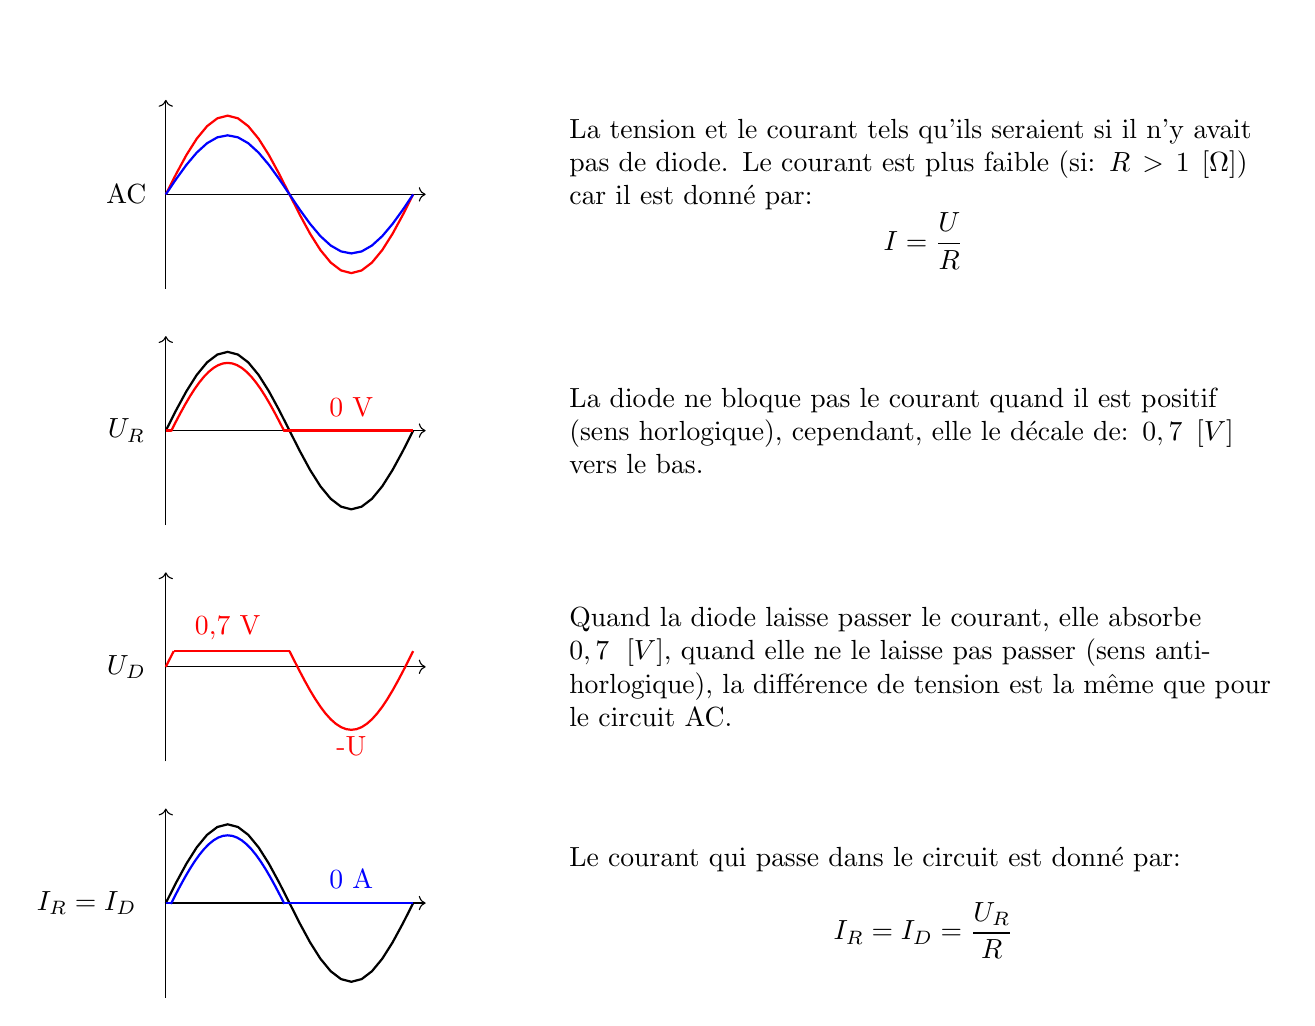
\begin{tikzpicture}
        \node [] at (0,2) {};

        %% courant alternatif normal
        \node [] at (-0.5,0) {AC};

        \draw [->] (0,-1.2) -- (0,1.2);
        \draw [->] (0,0) -- (3.30,0);
        \draw [thick, domain=0:pi, red] plot (\x,{sin(\x r * 2)});
        \draw [thick, domain=0:pi, blue] plot (\x,{0.75 * sin(\x r * 2)});

        \node [anchor=west, text width=9cm] at (5,0) {La tension et le courant tels qu'ils seraient si il n'y avait pas de diode. Le courant est plus faible (si: $ R > 1 \; [\Omega] $) car il est donné par: \[ I = \frac{U}{R} \]};

        %% tension dans la résistance
        \node [] at (-0.5,-3) {$ U_{R} $};

        \draw [->] (0,-4.2) -- (0,-1.8);
        \draw [->] (0,-3) -- (3.30,-3);
        \draw [yshift=-3cm, thick, domain=0:pi] plot (\x,{sin(\x r*2)});
        \draw [yshift=-3cm, thick, domain=0.13/2:pi/2-0.13/2, red] plot (\x,{sin(\x r*2)-0.14});
        \draw [yshift=-3cm, -, red, thick] (pi/2-0.13/2,0) -- (pi,0);
        \draw [yshift=-3cm, -, red, thick] (0,0) -- (0.13/2,0);
        \node [yshift=-3cm, red] at (3*pi/4, 0.3) {0 V};

        \node [anchor=west, text width=9cm] at (5,-3) {La diode ne bloque pas le courant quand il est positif (sens horlogique), cependant, elle le décale de: $ 0,7 \; [V] $ vers le bas.};

        %% tension dans la diode
        \node [] at (-0.5,-6) {$ U_{D} $};

        \draw [->] (0,-7.2) -- (0,-4.8);
        \draw [->] (0,-6) -- (3.30,-6);
        \draw [thick, domain=pi/2:pi, yshift=-6cm, red] plot (\x,{sin(\x r * 2) + 0.2});
        \draw [thick, domain=0:0.10, yshift=-6cm, red] plot (\x,{sin(\x r * 2)});
        \draw [thick, red, yshift=-6cm] (0.10,0.2) -- (pi/2,0.2);
        \node [yshift=-6cm, red] at (pi/4, 0.5) {0,7 V};
        \node [yshift=-6cm, red] at (3*pi/4, -1.0) {-U};

        \node [anchor=west, text width=9cm] at (5,-6) {Quand la diode laisse passer le courant, elle absorbe $ 0,7 \; [V] $, quand elle ne le laisse pas passer (sens anti-horlogique), la différence de tension est la même que pour le circuit AC.};

        %% courant dans le circuit
        \node [yshift=-9cm, anchor=east] at (-0.25,0) {$ I_R = I_D $};

        \draw [yshift=-9cm, ->] (0,-1.2) -- (0,1.2);
        \draw [yshift=-9cm, ->] (0,0) -- (3.30,0);
        \draw [yshift=-9cm, thick, domain=0:pi] plot (\x,{sin(\x r*2)});
        \draw [yshift=-9cm, thick, domain=0.13/2:pi/2-0.13/2, blue] plot (\x,{sin(\x r*2)-0.14});
        \draw [yshift=-9cm, -, blue, thick] (pi/2-0.13/2,0) -- (pi,0);
        \draw [yshift=-9cm, -, blue, thick] (0,0) -- (0.13/2,0);
        \node [yshift=-9cm, blue] at (3*pi/4, 0.3) {0 A};

        \node [yshift=-9cm, anchor=west, text width=9cm] at (5,0) {Le courant qui passe dans le circuit est donné par: \[ I_R = I_D = \frac{U_R}{R} \]};

    \end{tikzpicture}
\end{center}
Remarque: la somme de $ U_{R} $ et $ U_D $ donne le même graphe que AC.










\subsection{Redressement double alternance avec condensateur}





Circuit complet:
\begin{center}
    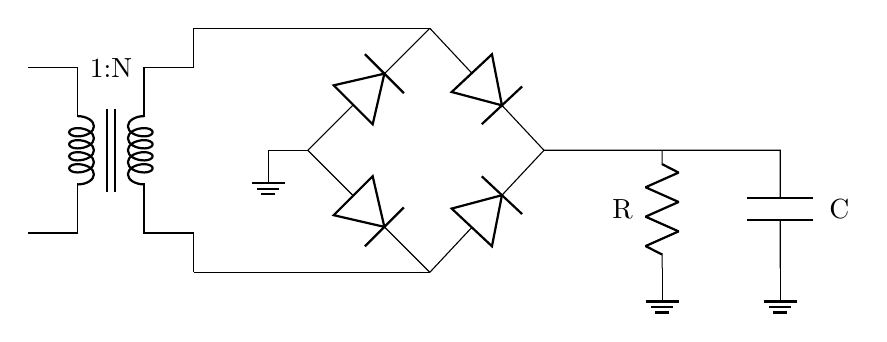
\begin{tikzpicture}

        \node (transfo) [transformer core] at (0,0) {};
        \node [] at (transfo.base) {1:N};

        \draw ($(transfo.B1) + (3, 0.5)$) to[diode] (1.5 + 4, 0);
        \draw ($(transfo.B2) + (3,-0.5)$) to[diode] (1.5 + 4, 0);
        \draw (-1.5 + 4, 0) to[diode] ($(transfo.B1) + (3, 0.5)$);
        \draw (-1.5 + 4, 0) to[diode] ($(transfo.B2) + (3,-0.5)$);

        \draw (transfo.B1) -- ($(transfo.B1) + (0, 0.5)$);
        \draw (transfo.B2) -- ($(transfo.B2) + (0,-0.5)$);
        \draw ($(transfo.B1) + (0, 0.5)$) -- ($(transfo.B1) + (3, 0.5)$);
        \draw ($(transfo.B2) + (0,-0.5)$) -- ($(transfo.B2) + (3,-0.5)$);

        \node (ground) [ground] at (2,0) {};
        \draw (ground) -- (-1.5 + 4, 0);

        \draw (1.5 + 4, 0) -- (8.5,0) to[capacitor] (8.5,-1.5) node[ground]{};
        \draw (7,0) to[resistor] (7,-1.5) node[ground]{};
        \node [anchor=east] at (6.75,-0.75) {R};
        \node [anchor=west] at (9,-0.75) {C};

    \end{tikzpicture}
\end{center}
Formules:
\begin{itemize}

    \item tension d'ondulation:
    \[
        V_{\text{o, càc}} = V_{max} - V_{min} = \frac{V_{ch, max}}{f R C}
    \]

    \item tension moyenne:
    \[
        V_{moy} = V_{ch, max} \times \bigg( 1 - \frac{1}{2 f R C} \bigg)
    \]

    \item coefficient d'ondulation:
    \[ \begin{aligned}
        r &= \frac{V_{\text{o, càc}}}{V_{moy}} = \frac{U_{max} - U_{min}}{V_{moy}} \\
        &= \frac{2}{2 f R C - 1}
    \end{aligned} \]

    \item condensateur:
    \[
        C = \frac{2 + r}{2 f R r}
    \]

\end{itemize}
\textbf{Remarque:} sans condensateur, on a bien: $\displaystyle V_{moy} = 2 \times \frac{V_{max}}{\pi} $.
\begin{center}
    \includegraphics[width=0.65\textwidth]{images/filtrage-condensateur.PNG}
\end{center}










\subsection{Transformateur électrique}





\begin{center}
    \begin{tabular}{cc|cc}
        Théorie:&&& Exemple:\\
        rapport de transformation=$\displaystyle \frac{N_2}{N_1}$&&&rapport de transformation = 3\\
        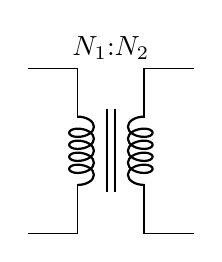
\begin{tikzpicture}
            \node (transfo) [transformer core] at (0,0) {};
            \node [yshift=0.25cm] at (transfo.base) {$N_1$:$N_2$};
        \end{tikzpicture}
        &
        \hspace{1cm} & \hspace{1cm}
        &
        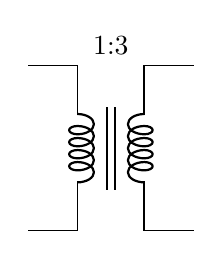
\begin{tikzpicture}
            \node (transfo) [transformer core] at (0,0) {};
            \node [yshift=0.25cm] at (transfo.base) {1:3};
        \end{tikzpicture}
    \end{tabular}
\end{center}
La tension qu'on obtient (à droite sur le schéma) est multipliée par le rapport de transformation.










\subsection{Diode}





\begin{center}
    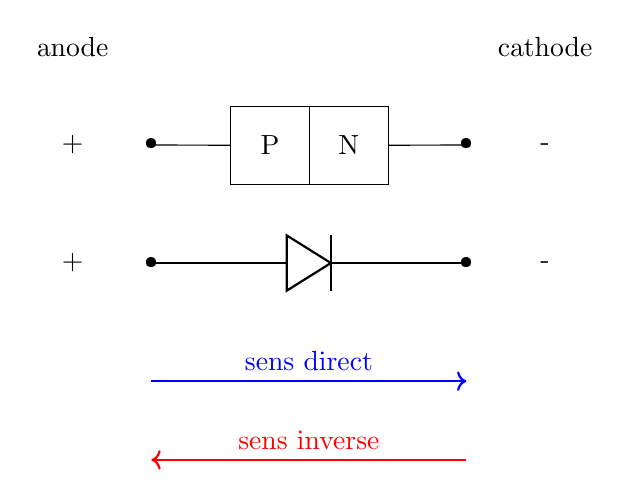
\begin{tikzpicture}
        \node (P) [rect, minimum width=1cm] at (0,0) {P};
        \node (N) [rect, minimum width=1cm] at (1,0) {N};

        \draw (-1,-0.5) node[]{\textbullet} -- (P);
        \draw (3,-0.5) node[]{\textbullet} -- (N);

        \draw (-1,-2) node[]{\textbullet} to[diode] (3,-2) node[]{\textbullet};

        \foreach \i in {0,1}
        {
            \node [] at (-2,-0.5-1.5*\i) {+};
            \node [] at (4,-0.5-1.5*\i) {-};
        }
        \node [] at (-2,0.75) {anode};
        \node [] at (4,0.75) {cathode};

        \draw [->, thick, blue] (-1,-3.5) -- node[anchor=south]{sens direct} (3,-3.5);
        \draw [<-, thick, red] (-1,-4.5) -- node[anchor=south]{sens inverse} (3,-4.5);
    \end{tikzpicture}
    \includegraphics[width=0.45\textwidth]{images/polarisation-directe01.png}
\end{center}

La diode est une jonction PN qui ne conduit le courant que lorsqu'elle est en polarisation directe et si la tension est plus élevée que la tension de seuil (0,7 V pour les diodes au silicium et 0,3 V pour les diodes au germanium).










\subsection{Transistor}





\begin{center}
    \begin{tikzpicture}

        \node (npn) [npn] at (-4.5,-0.5) {};

        \node [red] at (npn.B) {\textbullet};
        \node [red] at (npn.C) {\textbullet};
        \node [red] at (npn.E) {\textbullet};

        \node [anchor=east, red, xshift=-0.2cm] at (npn.B) {base};
        \node [anchor=west, red, xshift=0.2cm] at (npn.C) {collecteur};
        \node [anchor=west, red, xshift=0.2cm] at (npn.E) {émetteur};

        %% NPN

        \node (N1) [rect, minimum width=1cm] at (0,1) {P};
        \node (P) [rect, minimum width=1cm] at (0,0) {N};
        \node (N) [rect, minimum width=1cm] at (0,-1) {P};

        \draw (0.5,-2.5) node[]{\textbullet} -- (N);
        \draw (0.5,1.5) node[]{\textbullet} -- (N1);
        \draw (-0.5,-0.5) node[]{\textbullet} -- (P);

        \node [anchor=east, red, xshift=-0.2cm] at (-0.5,-0.5) {B};
        \node [anchor=south, red, yshift=0.2cm] at (0.5,1.5) {C};
        \node [anchor=north, red, yshift=-0.2cm] at (0.5,-2.5) {E};

        %% courants

        \node (npn) [npn] at (4.5,-0.5) {};

        \draw[<-, xshift=4.5cm] (npn.B) -- node[anchor=south]{$ I_B $} ($(npn.B) + (-0.5,0)$);
        \draw[<-, xshift=4.5cm] (npn.C) -- node[anchor=west]{$ I_C $} ($(npn.C) + (0,0.5)$);
        \draw[>-, xshift=4.5cm] (npn.E) -- node[anchor=west]{$ I_E $} ($(npn.E) + (0,-0.5)$);

    \end{tikzpicture}
\end{center}
\[ I_E = I_B + I_C \]
Le transistor a 3 états:
\begin{itemize}
    \item bloqué ($ I_b < I_c \quad \& \quad I_b \approx 0 $),
    \item saturé ($ I_b > I_c \quad \& \quad I_c \approx 0 $),
    \item linéaire.
\end{itemize}
Quand l'état est linéaire, le circuit est fermé et le courant passe normalement.

\begin{center}
    \begin{tikzpicture}
        \node (N1) [rect, minimum width=1cm] at (0,1) {N};
        \node (P) [rect, minimum width=1cm] at (0,0) {P};
        \node (N) [rect, minimum width=1cm] at (0,-1) {N};

        \draw (0.5,-2.5) node[]{\textbullet} -- (N);
        \draw (0.5,1.5) node[]{\textbullet} -- (N1);
        \draw (-0.5,-0.5) node[]{\textbullet} -- (P);

        \node [anchor=east, red, xshift=-0.2cm] at (-0.5,-0.5) {B};
        \node [anchor=south, yshift=0.2cm] at (0.5,1.5) {C};
        \node [anchor=north, red, yshift=-0.2cm] at (0.5,-2.5) {E};

        \node (npn) [npn, anchor=west] at (2.5,-0.5) {};

        \node [] at (npn.B) {\textbullet};
        \node [] at (npn.C) {\textbullet};
        \node [] at (npn.E) {\textbullet};

        \node [anchor=east, red, xshift=-0.2cm] at (npn.B) {B};
        \node [anchor=south, yshift=0.2cm] at (npn.C) {C};
        \node [anchor=north, red, yshift=-0.2cm] at (npn.E) {E};
    \end{tikzpicture}
    \hspace{4cm}
    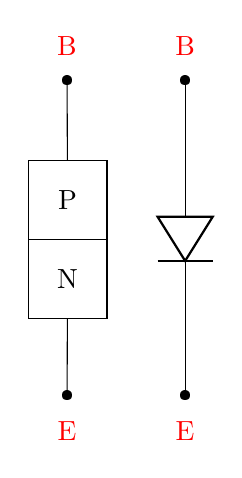
\begin{tikzpicture}
        \node (P) [rect, minimum width=1cm] at (0,0) {P};
        \node (N) [rect, minimum width=1cm] at (0,-1) {N};

        \draw (0.5,1) node[]{\textbullet} -- (P);
        \draw (0.5,-3) node[]{\textbullet} -- (N);

        \draw (2,1) node[]{\textbullet} to[diode] (2,-3) node[]{\textbullet};

        \node [anchor=south, red, yshift=0.2cm] at (0.5,1) {B};
        \node [anchor=north, red, yshift=-0.2cm] at (0.5,-3) {E};
        \node [anchor=south, red, yshift=0.2cm] at (2,1) {B};
        \node [anchor=north, red, yshift=-0.2cm] at (2,-3) {E};
    \end{tikzpicture}
\end{center}
\textbf{Remarque:} le courant qui passe de la base à l'émetteur (de B à E) traverse une jonction P puis une jonction N, comme si il passait à travers une diode. La tension entre B et E est donc de 0,7 V, comme pour une diode.

\begin{center}
    \textcolor{purple}{\textbf{Que représentent $ \alpha_{cc} $ et $ \beta_{cc} $ ?}}
    \textcolor{purple}{\textbf{Comment les calculer ?}}
\end{center}
Il y a 2 coefficients importants qui caractérisent les transistors:
\begin{itemize}
    \item $ \alpha_{cc} $ est le ratio entre le courant qui entre dans le transistor ($ I_C $) et le courant qui en sort ($ I_E $).
    \item $ \beta_{cc} $ représente un gain de courant, c'est le ratio du courant commandé ($ I_C $) par le courant qui commande la fermeture du transistor ($ I_B $).
\end{itemize}
\[
    \alpha_{cc} = \frac{I_C}{I_E}
    \qquad
    \beta_{cc} = \frac{I_C}{I_B}
\]
Rapports entre $ \alpha_{cc} $ et $ \beta_{cc} $:
\[
    \alpha_{cc} = \frac{\beta_{cc}}{\beta_{cc} + 1}
    \qquad
    \beta_{cc} = \frac{\alpha_{cc}}{1 - \alpha_{cc}}
\]















\section{Examen 2019}





\begin{enumerate}




\item Lorqu'elle est en polarisation directe, une diode:
\begin{enumerate}
    \item bloque le courant,
    \item conduit le courant,
    \item offre une forte résistance,
    \item absorbe une forte tension.
\end{enumerate}
\begin{example}
    \textbf{(b)}
    \begin{center}
        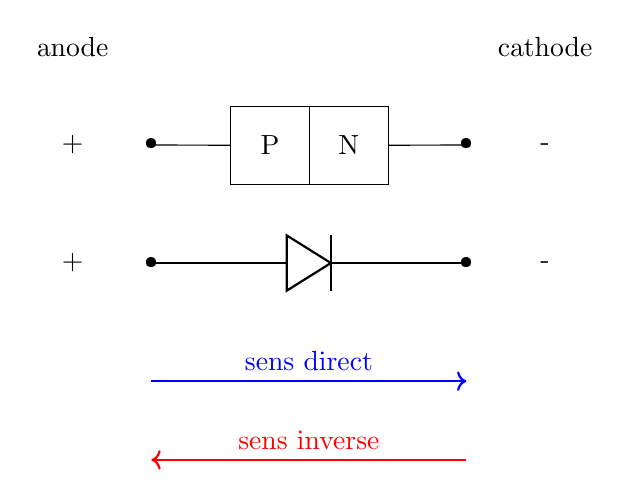
\begin{tikzpicture}
            \node (P) [rect, minimum width=1cm] at (0,0) {P};
            \node (N) [rect, minimum width=1cm] at (1,0) {N};

            \draw (-1,-0.5) node[]{\textbullet} -- (P);
            \draw (3,-0.5) node[]{\textbullet} -- (N);

            \draw (-1,-2) node[]{\textbullet} to[diode] (3,-2) node[]{\textbullet};

            \foreach \i in {0,1}
            {
                \node [] at (-2,-0.5-1.5*\i) {+};
                \node [] at (4,-0.5-1.5*\i) {-};
            }
            \node [] at (-2,0.75) {anode};
            \node [] at (4,0.75) {cathode};

            \draw [->, thick, blue] (-1,-3.5) -- node[anchor=south]{sens direct} (3,-3.5);
            \draw [<-, thick, red] (-1,-4.5) -- node[anchor=south]{sens inverse} (3,-4.5);
        \end{tikzpicture}
        \includegraphics[width=0.45\textwidth]{images/polarisation-directe01.png}
    \end{center}

    Lorsqu'elle est en polarisation directe, la diode conduit le courant à partir de la tension de seuil (0,7 V pour le silicium).
\end{example}





\item Une diode au silicium est en série avec une source de tension de 5 V et une résistance de 100 $ \Omega $. Si l'anode est branchée à la borne positive, la tension entre la cathode et la borne négative de la source sera de:
\begin{enumerate}
    \item 0,7 V
    \item 0,3 V
    \item 5,7 V
    \item 4,3 V
\end{enumerate}
\begin{example}
    \textbf{(d)}
    \begin{center}
        \begin{circuitikz}
            \draw (3,0) to[battery1=5 V] (0,0);
            \draw (3,0) to[diode] (3,-2);
            \draw (3,-2) to[R=$ 100 \; \Omega $] (0,-2);
            \draw (0,-2) -- (0,0);
        \end{circuitikz}
        \qquad \qquad
        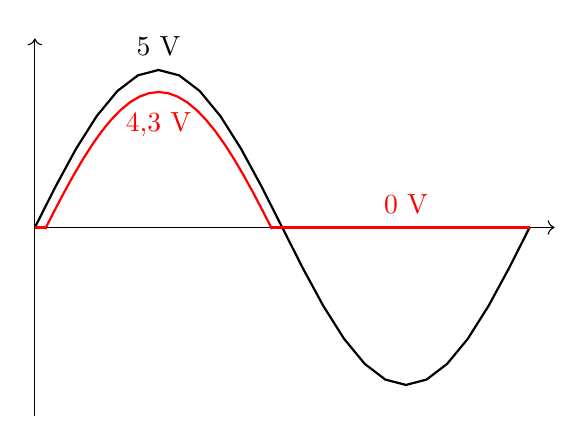
\begin{tikzpicture}
            \draw [->] (0,-2.4) -- (0,2.4);
            \draw [->] (0,0) -- (6.60,0);
            \draw [thick, domain=0:2*pi] plot (\x,{2*sin(\x r)});
            \draw [thick, domain=0.13:pi-0.13, red] plot (\x,{2*sin(\x r)-0.28});
            \draw [-, red, thick] (pi-0.13,0) -- (2*pi,0);
            \draw [-, red, thick] (0,0) -- (0.13,0);

            \node [] at (pi/2,2.3) {5 V};
            \node [red] at (pi/2,1.3) {4,3 V};
            \node [red] at (3*pi/2, 0.3) {0 V};
        \end{tikzpicture}
    \end{center}

    La diode en silicium a une tension de seuil de 0,7 V. La tension mesurée entre la cathode et la borne négative de la source sera donc de 4,3 V (= 5 - 0,7).
\end{example}





\item La polarisation inverse d'une jonction PN est obtenue en:
\begin{enumerate}
    \item \label{polar1} appliquant une tension externe positive à l'anode et négative à la cathode,
    \item appliquant une tension externe positive à la cathode et négative à l'anode,
    \item \label{polar3} appliquant une tension externe positive à la région P et négative à la région N,
    \item les réponses \ref{polar1} et \ref{polar3}.
\end{enumerate}
\begin{example}
    \textbf{(b)}
    \begin{center}
        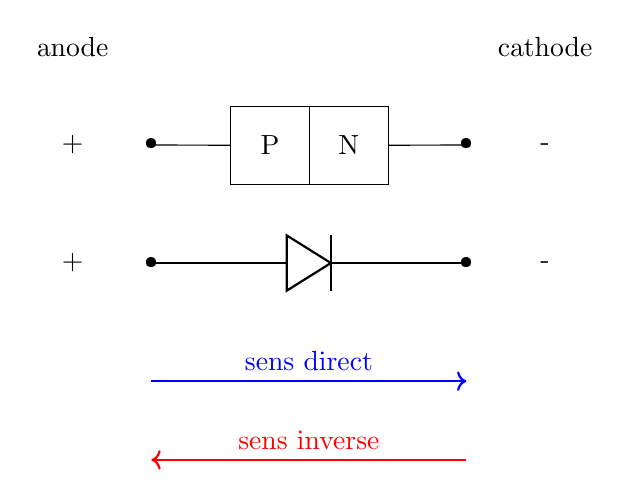
\begin{tikzpicture}
            \node (P) [rect, minimum width=1cm] at (0,0) {P};
            \node (N) [rect, minimum width=1cm] at (1,0) {N};

            \draw (-1,-0.5) node[]{\textbullet} -- (P);
            \draw (3,-0.5) node[]{\textbullet} -- (N);

            \draw (-1,-2) node[]{\textbullet} to[diode] (3,-2) node[]{\textbullet};

            \foreach \i in {0,1}
            {
                \node [] at (-2,-0.5-1.5*\i) {+};
                \node [] at (4,-0.5-1.5*\i) {-};
            }
            \node [] at (-2,0.75) {anode};
            \node [] at (4,0.75) {cathode};

            \draw [->, thick, blue] (-1,-3.5) -- node[anchor=south]{sens direct} (3,-3.5);
            \draw [<-, thick, red] (-1,-4.5) -- node[anchor=south]{sens inverse} (3,-4.5);
        \end{tikzpicture}
    \end{center}
\end{example}





\item La valeur moyenne d'une tension redressée simple alternance d'une valeur de crête de 200 V est:
\begin{enumerate}
    \item 63,7 V
    \item 127,3 V
    \item 141 V
    \item 0 V
\end{enumerate}
\begin{example}
    \textbf{(a)}
    \[ U_{moy} = \frac{U_{\text{crête}}}{\pi} = \frac{200}{\pi} = 63,66 \approx 63,7 \]
\end{example}





\item La valeur moyenne d'une tension redressée double alternance d'une valeur de crête de 100 V est:
\begin{enumerate}
    \item 63,7 V
    \item 127,3 V
    \item 141 V
    \item 0 V
\end{enumerate}
\begin{example}
    \textbf{(a)}
    \[ U_{moy} = \frac{2 \times U_{\text{crête}}}{\pi} = \frac{2 \times 100}{\pi} = 63,66 \approx 63,7 \]
\end{example}





\item La valeur de crête à l'entrée d'un redresseur une alternance est de 10 V. La valeur de crête à la sortie est de:
\begin{enumerate}
    \item 10 V
    \item 10,7 V
    \item 9,3 V
    \item 3,18 V
\end{enumerate}
\begin{example}
    \textbf{(c)} 10 - 0,7 = 9,3 V, car la tension de seuil d'une diode en silicium est de 0,7 V.
\end{example}





\item Dans un transistor, le courant $ I_C $ est le plus important, vrai ou faux ?
\begin{example}
    \textbf{Faux.}
    \begin{center}
        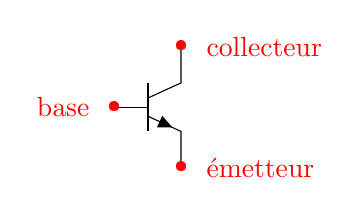
\begin{tikzpicture}

            \node (npn) [npn] at (0,0) {};

            \node [red] at (npn.B) {\textbullet};
            \node [red] at (npn.C) {\textbullet};
            \node [red] at (npn.E) {\textbullet};

            \node [anchor=east, red, xshift=-0.2cm] at (npn.B) {base};
            \node [anchor=west, red, xshift=0.2cm] at (npn.C) {collecteur};
            \node [anchor=west, red, xshift=0.2cm] at (npn.E) {émetteur};

        \end{tikzpicture}
        \qquad \qquad
        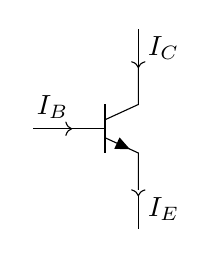
\begin{tikzpicture}

            \node (npn) [npn] at (0,0) {};

            \draw[<-] (npn.B) -- node[anchor=south]{$ I_B $} ($(npn.B) + (-0.5,0)$);
            \draw[<-] (npn.C) -- node[anchor=west]{$ I_C $} ($(npn.C) + (0,0.5)$);
            \draw[>-] (npn.E) -- node[anchor=west]{$ I_E $} ($(npn.E) + (0,-0.5)$);

        \end{tikzpicture}
        \qquad \qquad
        \[ I_E = I_B + I_C \quad \implies \quad I_E > I_C \]
    \end{center}
\end{example}





\item La chute de tension entre la base et le collecteur d'un transistor est toujours égale à 0,7 V quand le transistor est passant, vrai ou faux ?
\begin{example}
    \textbf{Vrai.}
    \begin{center}
        \includegraphics[width=0.90\textwidth]{images/transistor-VBE.PNG}
    \end{center}

    \textbf{Remarque:} le courant qui passe de la base à l'émetteur (de B à E) traverse une jonction P puis une jonction N, comme si il passait à travers une diode. La tension entre B et E est donc de 0,7 V, comme pour une diode.

    \begin{center}
        \begin{tikzpicture}
            \node (N1) [rect, minimum width=1cm] at (0,1) {N};
            \node (P) [rect, minimum width=1cm] at (0,0) {P};
            \node (N) [rect, minimum width=1cm] at (0,-1) {N};

            \draw (0.5,-2.5) node[]{\textbullet} -- (N);
            \draw (0.5,1.5) node[]{\textbullet} -- (N1);
            \draw (-0.5,-0.5) node[]{\textbullet} -- (P);

            \node [anchor=east, red, xshift=-0.2cm] at (-0.5,-0.5) {B};
            \node [anchor=south, yshift=0.2cm] at (0.5,1.5) {C};
            \node [anchor=north, red, yshift=-0.2cm] at (0.5,-2.5) {E};

            \node (npn) [npn, anchor=west] at (2.5,-0.5) {};

            \node [] at (npn.B) {\textbullet};
            \node [] at (npn.C) {\textbullet};
            \node [] at (npn.E) {\textbullet};

            \node [anchor=east, red, xshift=-0.2cm] at (npn.B) {B};
            \node [anchor=south, yshift=0.2cm] at (npn.C) {C};
            \node [anchor=north, red, yshift=-0.2cm] at (npn.E) {E};
        \end{tikzpicture}
        \hspace{4cm}
        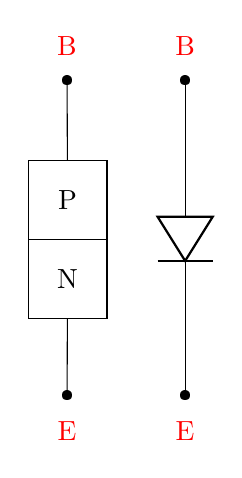
\begin{tikzpicture}
            \node (P) [rect, minimum width=1cm] at (0,0) {P};
            \node (N) [rect, minimum width=1cm] at (0,-1) {N};

            \draw (0.5,1) node[]{\textbullet} -- (P);
            \draw (0.5,-3) node[]{\textbullet} -- (N);

            \draw (2,1) node[]{\textbullet} to[diode] (2,-3) node[]{\textbullet};

            \node [anchor=south, red, yshift=0.2cm] at (0.5,1) {B};
            \node [anchor=north, red, yshift=-0.2cm] at (0.5,-3) {E};
            \node [anchor=south, red, yshift=0.2cm] at (2,1) {B};
            \node [anchor=north, red, yshift=-0.2cm] at (2,-3) {E};
        \end{tikzpicture}
    \end{center}
\end{example}





\item Le rapport de $ I_E $ sur $ I_B $ est égal à $ \beta_{cc} $, vrai ou faux ?
\begin{example}
    \textbf{Faux.}
    \[ \beta_{cc} = \frac{I_C}{I_B} \qquad \qquad \qquad \alpha_{cc} = \frac{I_C}{I_E} \]
\end{example}





\item Si $ I_C $ est 50 fois plus élevé que $ I_B $, la valeur de $ \beta_{cc} $ vaut 50, vrai ou faux ?
\begin{example}
    \textbf{Vrai.}
    \[ I_C = 50 \times I_B \quad \implies \quad \beta_{cc} = \frac{I_C}{I_B} = \frac{50 \times I_B}{I_B} = 50 \]
\end{example}





\item Si la valeur de $ \beta_{cc} $ est de 100, la valeur de $ \alpha_{cc} $ est de 0,01, vrai ou faux ?
\begin{example}
    \textbf{Faux.}
    \[ \alpha_{cc} = \frac{I_C}{I_E} = \frac{\beta_{cc}}{\beta_{cc} + 1} = \frac{100}{101} \approx 0.99 \neq 0.01 \]
\end{example}





\item Dans un transistor, le courant de base est égal à 2 \% du courant de l'émetteur qui est de 30 mA. Déterminer le courant de collecteur.
\begin{example}
    \[ I_B = 0,02 \times I_E \; ; \quad I_E = 30 \; [mA] \; ; \quad I_E = I_C + I_B \]
    \[ \implies I_C = I_E - I_B = 30 - 0,02 \times 30 = 29,4 \; [mA] \]
    \[ \fbox{$\displaystyle I_C = 29,4 \; [mA] $} \]
\end{example}





\item Quelle sera la valeur de $ \beta_{cc} $ lorsque $ I_E $ = 25 mA et $ I_B $ = 200 mA ?
\begin{example}
    \[ \beta_{cc} = \frac{I_C}{I_B} \; ; \quad I_E = I_C + I_B \quad \implies \quad \beta_{cc} = \frac{I_E - I_B}{I_B} = \frac{25 - 200}{200} = -0,875 \; [mA] \]
    \[ \fbox{$\displaystyle \beta_{cc} = -0,875 \; [mA] $} \]

    \textbf{Remarque:} il y a un problème avec la question. Normalement, vu que: $ I_E = I_B + I_C $, on a: $ I_E > I_B $, ce qui n'est pas le cas ici.
\end{example}





\item Si un transistor possède une valeur de $ \alpha_{cc} = 0,96 $; déterminer $ I_C $ lorsque $ I_E = 9,35 $ mA.
\begin{example}
    \[ I_E = 9,35 \; [mA] \; \quad \alpha_{cc} = \frac{I_C}{I_E} = 0,96 \implies I_C = \alpha_{cc} \times I_E = 0,96 \times 9,35 = 8,98 \; [mA] \]
    \[ \fbox{$\displaystyle I_C = 8,98 \; [mA] $} \]
\end{example}





\item \label{QPontRedresseur1} Pour un pont redresseur connecté au réseau, quelle sera la fréquence de sortie ?
\begin{example}
    La fréquence du réseau est de 50 Hz. Le pont redresseur va doubler la fréquence, donc 100 Hz.
    \begin{center}
        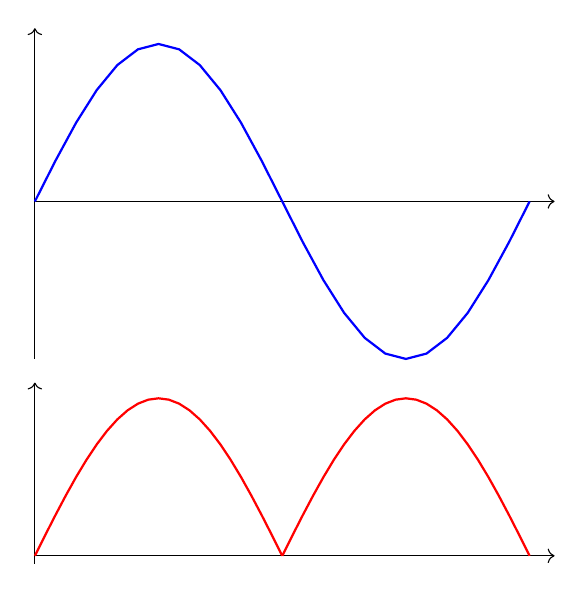
\begin{tikzpicture}
            \draw [->] (0,-2) -- (0,2.2);
            \draw [->] (0,0) -- (6.60,0);
            \draw [thick, blue, domain=0:2*pi] plot (\x,{2*sin(\x r)});

            \draw [->, yshift=-4.5cm] (0,-0.1) -- (0,2.2);
            \draw [->, yshift=-4.5cm] (0,0) -- (6.60,0);
            \draw [thick, red, domain=0:pi, yshift=-4.5cm] plot (\x,{2*sin(\x r)});
            \draw [thick, red, domain=pi:2*pi, yshift=-4.5cm] plot (\x,{2*sin((\x+pi) r)});
        \end{tikzpicture}
    \end{center}
    \[ \fbox{$f_s = 100 \; [Hz]$} \]
\end{example}





\item \label{QPontRedresseur2} Pour ce même pont redresseur (Q \ref{QPontRedresseur1}), quelle sera le tension de crête au secondaire sachant que le rapport de transformation vaut 3 ?
\begin{example}
    La tension du réseau vaut 230 V. La tension de sortie sera donc: $\displaystyle 230 \times 3 = 690 $ V.
    \begin{center}
        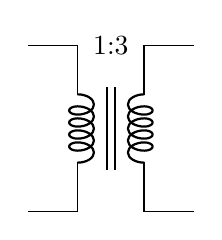
\begin{tikzpicture}
            \node (transfo) [transformer core] at (0,0) {};
            \node [] at (transfo.base) {1:3};
        \end{tikzpicture}
    \end{center}
    \[ \fbox{$V_s = 690 \; [V]$} \]
\end{example}





\item Pour ce même pont redresseur (Q \ref{QPontRedresseur1} et \ref{QPontRedresseur2}), quelle valeur doit avoir le condensateur pour avoir un r = 2 \%, si R = 3 k$ \Omega $ ?
\begin{example}
    Circuit complet:
    \begin{center}
        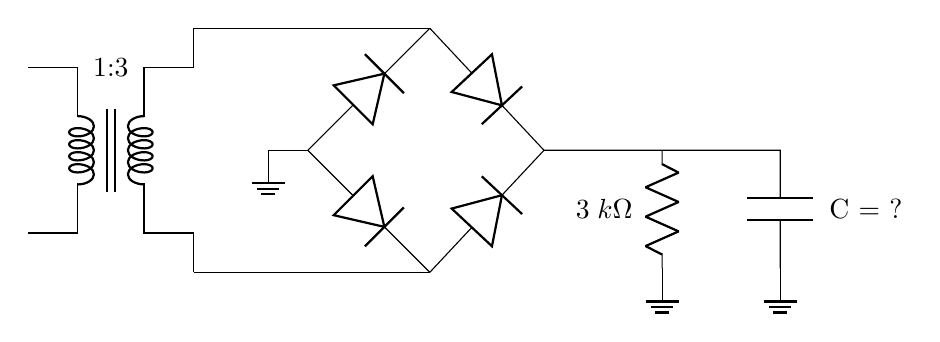
\begin{tikzpicture}

            \node (transfo) [transformer core] at (0,0) {};
            \node [] at (transfo.base) {1:3};

            \draw ($(transfo.B1) + (3, 0.5)$) to[diode] (1.5 + 4, 0);
            \draw ($(transfo.B2) + (3,-0.5)$) to[diode] (1.5 + 4, 0);
            \draw (-1.5 + 4, 0) to[diode] ($(transfo.B1) + (3, 0.5)$);
            \draw (-1.5 + 4, 0) to[diode] ($(transfo.B2) + (3,-0.5)$);

            \draw (transfo.B1) -- ($(transfo.B1) + (0, 0.5)$);
            \draw (transfo.B2) -- ($(transfo.B2) + (0,-0.5)$);
            \draw ($(transfo.B1) + (0, 0.5)$) -- ($(transfo.B1) + (3, 0.5)$);
            \draw ($(transfo.B2) + (0,-0.5)$) -- ($(transfo.B2) + (3,-0.5)$);

            \node (ground) [ground] at (2,0) {};
            \draw (ground) -- (-1.5 + 4, 0);

            \draw (1.5 + 4, 0) -- (8.5,0) to[capacitor] (8.5,-1.5) node[ground]{};
            \draw (7,0) to[resistor] (7,-1.5) node[ground]{};
            \node [anchor=east] at (6.75,-0.75) {$3 \; k \Omega$};
            \node [anchor=west] at (9,-0.75) {C = ?};

        \end{tikzpicture}
    \end{center}
    Tension:
    \begin{center}
        \includegraphics[width=0.65\textwidth]{images/filtrage-condensateur.PNG}
    \end{center}
    Calcul:
    \[
        C = \frac{2 + r}{2 f R r}
        = \frac{2 + 0,02}{2 \times 100 \; [Hz] \times 3000 \; [\Omega] \times 0,02}
        = 0,000168333333 \; [F]
    \]
    \[ \fbox{$C = 168 \; [\mu F]$} \]
\end{example}





\item Quelle est la puissance dissipée dans une diode parcourue par un courant de 100 mA ?
\begin{example}
    \[ U_{diode} = 0,7 \; [V] \; ; \quad I = 100 \; [mA] = 0,1 \; [A] \; ; \quad P = U \times I = 0,07 \; [W] \]
    \[ \fbox{$\displaystyle P = 0,07 \; [W] $} \]
\end{example}





\item Les régions de type P d'un transistor PNP sont:
\begin{enumerate}
    \item base émetteur,
    \item base collecteur,
    \item émetteur collecteur.
\end{enumerate}
\begin{example}
    \textbf{(c)}

    \begin{center}
        \begin{tikzpicture}

            \node (npn) [npn] at (-4,-0.5) {};

            \node [red] at (npn.B) {\textbullet};
            \node [red] at (npn.C) {\textbullet};
            \node [red] at (npn.E) {\textbullet};

            \node [anchor=east, red, xshift=-0.2cm] at (npn.B) {base};
            \node [anchor=west, red, xshift=0.2cm] at (npn.C) {collecteur};
            \node [anchor=west, red, xshift=0.2cm] at (npn.E) {émetteur};

            %% NPN

            \node (N1) [rect, minimum width=1cm] at (0,1) {P};
            \node (P) [rect, minimum width=1cm] at (0,0) {N};
            \node (N) [rect, minimum width=1cm] at (0,-1) {P};

            \draw (0.5,-2.5) node[]{\textbullet} -- (N);
            \draw (0.5,1.5) node[]{\textbullet} -- (N1);
            \draw (-0.5,-0.5) node[]{\textbullet} -- (P);

            \node [anchor=east, red, xshift=-0.2cm] at (-0.5,-0.5) {B};
            \node [anchor=south, red, yshift=0.2cm] at (0.5,1.5) {C};
            \node [anchor=north, red, yshift=-0.2cm] at (0.5,-2.5) {E};

        \end{tikzpicture}
    \end{center}
\end{example}





\item Que vaut $ I_C $ quand le transistor est saturé ?
\begin{example}
    Le transistor a 2 états:
    \begin{itemize}
        \item bloqué,
        \item saturé.
    \end{itemize}
    Quand l'état est bloqué, le courant ne passe pas et $ I_C = 0 $. Quand l'état est saturé, le courant passe et $ I_C = I_E - I_B $.
    \[ \fbox{$I_C = I_E - I_B$} \]
\end{example}





\end{enumerate}















\section{Interro}





\begin{enumerate}





\item Les régions de type N d’un transistor NPN sont:
\begin{enumerate}
    \item base émetteur
    \item base collecteur
    \item émetteur collecteur
\end{enumerate}
\begin{example}
    \textbf{(c)}

    \begin{center}
        \begin{tikzpicture}

            \node (npn) [npn] at (-4,-0.5) {};

            \node [red] at (npn.B) {\textbullet};
            \node [red] at (npn.C) {\textbullet};
            \node [red] at (npn.E) {\textbullet};

            \node [anchor=east, red, xshift=-0.2cm] at (npn.B) {base};
            \node [anchor=west, red, xshift=0.2cm] at (npn.C) {collecteur};
            \node [anchor=west, red, xshift=0.2cm] at (npn.E) {émetteur};

            %% NPN

            \node (N1) [rect, minimum width=1cm] at (0,1) {N};
            \node (P) [rect, minimum width=1cm] at (0,0) {P};
            \node (N) [rect, minimum width=1cm] at (0,-1) {N};

            \draw (0.5,-2.5) node[]{\textbullet} -- (N);
            \draw (0.5,1.5) node[]{\textbullet} -- (N1);
            \draw (-0.5,-0.5) node[]{\textbullet} -- (P);

            \node [anchor=east, red, xshift=-0.2cm] at (-0.5,-0.5) {B};
            \node [anchor=south, red, yshift=0.2cm] at (0.5,1.5) {C};
            \node [anchor=north, red, yshift=-0.2cm] at (0.5,-2.5) {E};

        \end{tikzpicture}
    \end{center}
\end{example}





\item La tension aux bornes d’une jonction BE d’un transistor au silicium en fonctionnement normal est d’environ:
\begin{enumerate}
    \item 0 V
    \item 0,7 V
    \item 0,3 V
    \item indéterminée
\end{enumerate}
\begin{example}
    \textbf{(b)}

    Le courant qui passe de la base à l'émetteur (de B à E) traverse une jonction P puis une jonction N, comme si il passait à travers une diode. La tension entre B et E est donc de 0,7 V, comme pour une diode.

    \begin{center}
        \begin{tikzpicture}
            \node (N1) [rect, minimum width=1cm] at (0,1) {N};
            \node (P) [rect, minimum width=1cm] at (0,0) {P};
            \node (N) [rect, minimum width=1cm] at (0,-1) {N};

            \draw (0.5,-2.5) node[]{\textbullet} -- (N);
            \draw (0.5,1.5) node[]{\textbullet} -- (N1);
            \draw (-0.5,-0.5) node[]{\textbullet} -- (P);

            \node [anchor=east, red, xshift=-0.2cm] at (-0.5,-0.5) {B};
            \node [anchor=south, yshift=0.2cm] at (0.5,1.5) {C};
            \node [anchor=north, red, yshift=-0.2cm] at (0.5,-2.5) {E};

            \node (npn) [npn, anchor=west] at (2.5,-0.5) {};

            \node [] at (npn.B) {\textbullet};
            \node [] at (npn.C) {\textbullet};
            \node [] at (npn.E) {\textbullet};

            \node [anchor=east, red, xshift=-0.2cm] at (npn.B) {B};
            \node [anchor=south, yshift=0.2cm] at (npn.C) {C};
            \node [anchor=north, red, yshift=-0.2cm] at (npn.E) {E};
        \end{tikzpicture}
        \hspace{4cm}
        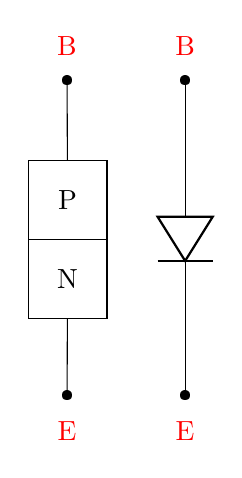
\begin{tikzpicture}
            \node (P) [rect, minimum width=1cm] at (0,0) {P};
            \node (N) [rect, minimum width=1cm] at (0,-1) {N};

            \draw (0.5,1) node[]{\textbullet} -- (P);
            \draw (0.5,-3) node[]{\textbullet} -- (N);

            \draw (2,1) node[]{\textbullet} to[diode] (2,-3) node[]{\textbullet};

            \node [anchor=south, red, yshift=0.2cm] at (0.5,1) {B};
            \node [anchor=north, red, yshift=-0.2cm] at (0.5,-3) {E};
            \node [anchor=south, red, yshift=0.2cm] at (2,1) {B};
            \node [anchor=north, red, yshift=-0.2cm] at (2,-3) {E};
        \end{tikzpicture}
    \end{center}
\end{example}





\item La valeur de crête à l’entrée d’un redresseur simple alternance est de 10 V. La valeur de crête approximative à la sortie est de:
\begin{enumerate}
    \item 10 V
    \item 3,18 V
    \item 10,7 V
    \item 9,3 V
\end{enumerate}
\begin{example}
    \textbf{(d)}

    \begin{center}
        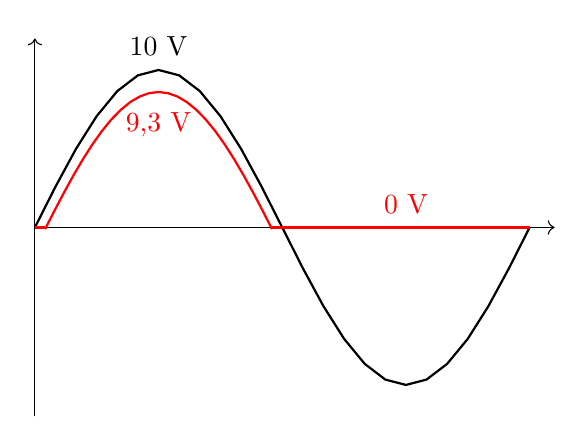
\begin{tikzpicture}
            \draw [->] (0,-2.4) -- (0,2.4);
            \draw [->] (0,0) -- (6.60,0);
            \draw [thick, domain=0:2*pi] plot (\x,{2*sin(\x r)});
            \draw [thick, domain=0.13:pi-0.13, red] plot (\x,{2*sin(\x r)-0.28});
            \draw [-, red, thick] (pi-0.13,0) -- (2*pi,0);
            \draw [-, red, thick] (0,0) -- (0.13,0);

            \node [] at (pi/2,2.3) {10 V};
            \node [red] at (pi/2,1.3) {9,3 V};
            \node [red] at (3*pi/2, 0.3) {0 V};
        \end{tikzpicture}
    \end{center}

    La diode en silicium a une tension de seuil de 0,7 V. La tension mesurée entre la cathode et la borne négative de la source sera donc de 9,3 V (= 10 - 0,7).
\end{example}





\item Pour le circuit de la question 3, la diode devra pouvoir supporter une tension inverse de:
\begin{enumerate}
    \item 10 V
    \item 5 V
    \item 20 V
    \item 3,18 V
\end{enumerate}
\begin{example}
    \textbf{(a)}

    \begin{center}
        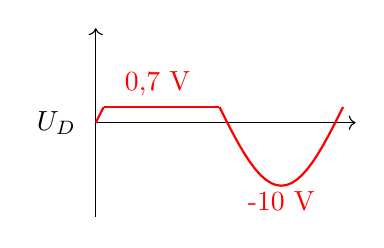
\begin{tikzpicture}
            %% tension dans la diode
            \node [] at (-0.5,-6) {$ U_{D} $};

            \draw [->] (0,-7.2) -- (0,-4.8);
            \draw [->] (0,-6) -- (3.30,-6);
            \draw [thick, domain=pi/2:pi, yshift=-6cm, red] plot (\x,{sin(\x r * 2) + 0.2});
            \draw [thick, domain=0:0.10, yshift=-6cm, red] plot (\x,{sin(\x r * 2)});
            \draw [thick, red, yshift=-6cm] (0.10,0.2) -- (pi/2,0.2);
            \node [yshift=-6cm, red] at (pi/4, 0.5) {0,7 V};
            \node [yshift=-6cm, red] at (3*pi/4, -1.0) {-10 V};
        \end{tikzpicture}
    \end{center}
\end{example}





\item Lorsque la tension de crête de sortie d’un redresseur en pont est de 20 V, la TIC aux bornes de chaque diode est de:
\begin{enumerate}
    \item 20 V
    \item 21,4 V
    \item 20,7 V
    \item 19,3 V
\end{enumerate}
\begin{example}
    \textbf{(b)}

    \begin{center}
        \includegraphics[width=0.4\textwidth]{images/pont-graetz-1.PNG}
        \hspace{2cm}
        \includegraphics[width=0.4\textwidth]{images/pont-graetz-2.PNG}
    \end{center}
    À cause des deux diodes, la tension de crête perd 1,4 V. Il faut les rajouter pour trouver la TIC.
\end{example}





\item Une tension de crête redressée double alternance de 60 V est appliquée à l’entrée d’un filtre à condensateur. Si la fréquence de sortie est de 120 Hz, la charge de 10 k$\Omega$ et C = 10 mF, la tension d’ondulation est:
\begin{enumerate}
    \item 0,6 V
    \item 6 mV
    \item 5 mV
    \item 2,88 V
\end{enumerate}
\begin{example}
    \textbf{(c)}
    \begin{center}
        \includegraphics[width=0.65\textwidth]{images/filtrage-condensateur.PNG}
    \end{center}
    \[
        V_{\text{o, càc}} = V_{ch, max} \times \frac{1}{f R C}
        = 60 \; [V] \times \frac{1}{120 \; [Hz] \times 10000 \; [\Omega] \times 0.010 \; [F]}
        = 0,005 \; [V]
    \]
    \[ \fbox{$ V_{\text{o, càc}} = 5 \; [mV] $} \]
\end{example}





\item La puissance moyenne fournie à la charge en négligeant la chute de potentiel dans la diode pour le circuit suivant vaut:
\begin{enumerate}
    \item 13,36 W
    \item 8,18 W
    \item 3,32 W
    \item 6,64 W
\end{enumerate}
\begin{center}
    \includegraphics[width=0.4\textwidth]{images/interro1-ex7-1.PNG}
\end{center}
\begin{example}
    \textbf{(c)}

    On a:
    \begin{itemize}
        \item la tension = $\displaystyle U_{moy} = \frac{120 \times \sqrt{2}}{2 \times \pi} \approx 27 \; [V] $,
        \item la résistance = $ R = 220 \; [\Omega] $,
        \item la relation: $ U = R \times I $.
    \end{itemize}
    \[ \implies P = U \times I = \frac{U^2}{R} \approx 3.31 \; [W] \]
\end{example}





\item La tension de crête de sortie d’un redresseur en pont est de 28,3 V. Quelle est la TIC aux bornes des diodes ?
\begin{enumerate}
    \item 28,3 V
    \item 29 V
    \item 29,7 V
    \item 27,6 V
\end{enumerate}
\begin{example}
    \textbf{(c)}

    Rappel: TIC = tension inverse maximale = tension maximale que la diode peut prendre en sens inverse avant de claquer.

    Avec un pont redresseur, on enlève 1,4 V à $ U_{\text{crête}} $. Il faut donc ajouter 1,4 V à $ U_{\text{crête}} $ pour connaître la TIC.
\end{example}





\item Les valeurs des courants IB et IC pour le montage suivant sont:
\begin{enumerate}
    \item IC = 51 mA, IB = 0,7 mA
    \item IC = 51 mA, IB = 0,51 mA
    \item IC = 34 mA, IB = 0,34 mA
    \item IC = 34 mA, IB = 0,7 mA
\end{enumerate}
\begin{center}
    \includegraphics[width=0.4\textwidth]{images/interro1-ex9-1.PNG}
\end{center}
\begin{example}
    \textbf{(d)}

    Loi des mailles (maille de gauche):
    \[
        V_{bb} - I_b \times R_b - 0,7 \; [V] = 0
        \quad \implies \quad
        I_b = \frac{V_{bb} - 0,7 \; [V]}{R_b}
    \]
    \[ \implies I_b \approx 0.702 \; [mA] \]
    Loi des mailles (maille de droite):
    \[
        V_{cc} - R_c \times I_c - V_{ce} = 0
        \quad \implies \quad
        I_c = \frac{V_{cc} - 8 \; [V]}{R_c}
    \]
    \[ \implies I_c \approx 34 \; [mA] \]
\end{example}





\item Quelle est la valeur du condensateur à utiliser pour produire un coefficient d’ondulation de 1 \% pour un redresseur double alternance qui possède une résistance de charge de 1,5 $ k \Omega $. On supposera que le redresseur produit une tension de crête de sortie de 25 V et que la fréquence du signal d’entrée est de 50 Hz.
\begin{enumerate}
    \item 1,005 mF
    \item 0,67 mF
    \item 1,34 mF
    \item 2,68 mF
\end{enumerate}
\begin{example}
    \textbf{(c)}

    Tension:
    \begin{center}
        \includegraphics[width=0.65\textwidth]{images/filtrage-condensateur.PNG}
    \end{center}
    \[
        C = \frac{2 + r}{2 f R r}
        = \frac{2 + 0,01}{2 \times 50 \; [Hz] \times 1500 \; [\Omega] \times 0,01}
        = 0.00134 \; [F]
    \]
    \[ \fbox{$\displaystyle C = 1,34 \; [mF] $} \]
\end{example}





\item Soit un redresseur en pont avec filtrage qu’on alimente avec une tension alternative sinusoïdale de valeur crête 55 V à une fréquence de 50 Hz. Si la résistance en charge vaut 10 $ k \Omega $ et que la capacité du condensateur vaut $ 2,5 \times 10^{-5} $ F, le coefficient d’ondulation vaut:
\begin{enumerate}
    \item 8 \%
    \item 16 \%
    \item 2 \%
    \item 4 \%
\end{enumerate}
\begin{example}
    \textbf{(a)}
    \[
        r = \frac{2}{2 f R C - 1}
        = \frac{2}{2 \times 50 \; [Hz] \times 10000 \; [\Omega] \times \; 2,5 \times 10^{-5} [F] - 1}
        = 0.0833333333
    \]
    \[ \fbox{$\displaystyle r = 8 \; \% $} \]
\end{example}





\item Le transistor est en saturation signifie:
\begin{enumerate}
    \item Le transistor va brûler car on se rapproche du claquage.
    \item Le courant base est trop important, le transistor ne fonctionne plus normalement.
    \item Le courant collecteur atteint un maximum, le courant base peut encore augmenter.
    \item Les courants collecteur et base atteignent un maximum au-delà duquel le transistor claque.
\end{enumerate}
\begin{example}
    \textbf{(b)} Quand le transistor est saturé, $ I_b $ est grand et $ I_c $ est petit ce qui n'est pas "normal" pour le transistor.
\end{example}





\item Quelle sera la valeur de $ \beta_{cc} $ si IE = 5,34 mA et IB = 0,0475 mA ?
\begin{enumerate}
    \item 11,1
    \item 112
    \item 111
    \item 11,2
\end{enumerate}
\begin{example}
    \textbf{(c)}
    \[ 
        I_C = I_E - I_B
        \quad \implies \quad
        \beta_{cc} = \frac{I_C}{I_B} = \frac{I_E - I_B}{I_B} \approx 111
    \]
\end{example}





\item En supposant que $V_{CE}$(sat) = 0 V, déterminer la valeur du courant IC(sat) pour le schéma suivant.
\begin{enumerate}
    \item 0,43 mA
    \item 4,3 mA
    \item 0,5 mA
    \item 5 mA
\end{enumerate}
\begin{center}
    \includegraphics[width=0.4\textwidth]{images/interro1-ex14-1.PNG}
\end{center}
\begin{example}
    \textbf{(c)}

    Loi des mailles (maille de droite):
    \[
        5 \; [V] - I_c \times 10 \; [k\Omega] = 0
        \quad \implies \quad
        I_c = 0,50 \; [mA]
    \]
\end{example}





\item Dans la question 14, quelle valeur de courant IB faut-il pour atteindre la saturation ?
\begin{enumerate}
    \item 0,33 mA
    \item 0,033 mA
    \item 0,0033 mA
    \item 0,00033 mA
\end{enumerate}
\begin{example}
    \textbf{(c)}
    \[ I_b = \frac{I_c}{\beta_{cc}} = \frac{0,50}{150} \; [mA] = 0.00333333333 \; [mA] \]
\end{example}





\end{enumerate}




















\part{Laboratoires}















\section{Allumer une Led via un bouton poussoir}










\subsection{Explication bouton}





On mesure la tension sur la pin 2. Pour éviter le \textit{flottement}, c-à-d éviter que la valeur lue par la pin change tout le temps, on connecte la pin 2 à la masse avec une grosse résistance. La grosse résistance sert à éviter que tout le courant passe du 5V à la masse directement quand on appuie sur le bouton.

\begin{center}
    \begin{tikzpicture}
        \node (pin2) [circle, draw=black] at (0,0) {2};
        \node (V5) [] at (3,3) {+ 5 V};
        \node (V0) [] at (3,-3) {+ 0 V};
        \node (bullet) [] at (3,0) {\textbullet};

        \draw (pin2) -- (3,0);
        \draw (bullet) to[normal open switch] (V5.south);
        \draw (bullet) to[R=10 k$\Omega$] (V0.north);
    \end{tikzpicture}
\end{center}
\begin{center}
    \begin{tikzpicture}
        \node (N1) [rect, minimum width=1cm] at (0,1) {N};
        \node (P) [rect, minimum width=1cm] at (0,0) {P};
        \node (N) [rect, minimum width=1cm] at (0,-1) {N};

        \draw (0.5,-2.5) node[]{\textbullet} -- (N);
        \draw (0.5,1.5) node[]{\textbullet} -- (N1);
        \draw (-0.5,-0.5) node[]{\textbullet} -- (P);

        \node [anchor=east, red, xshift=-0.2cm] at (-0.5,-0.5) {B};
        \node [anchor=south, yshift=0.2cm] at (0.5,1.5) {C};
        \node [anchor=north, red, yshift=-0.2cm] at (0.5,-2.5) {E};

        \node (npn) [npn, anchor=west] at (2.5,-0.5) {};

        \node [] at (npn.B) {\textbullet};
        \node [] at (npn.C) {\textbullet};
        \node [] at (npn.E) {\textbullet};

        \node [anchor=east, red, xshift=-0.2cm] at (npn.B) {B};
        \node [anchor=south, yshift=0.2cm] at (npn.C) {C};
        \node [anchor=north, red, yshift=-0.2cm] at (npn.E) {E};
    \end{tikzpicture}
    \hspace{4cm}
    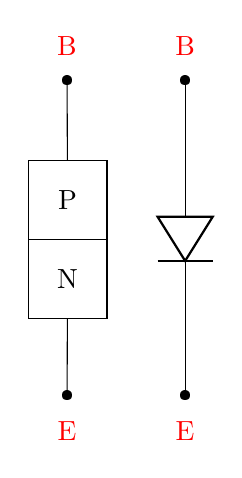
\begin{tikzpicture}
        \node (P) [rect, minimum width=1cm] at (0,0) {P};
        \node (N) [rect, minimum width=1cm] at (0,-1) {N};

        \draw (0.5,1) node[]{\textbullet} -- (P);
        \draw (0.5,-3) node[]{\textbullet} -- (N);

        \draw (2,1) node[]{\textbullet} to[diode] (2,-3) node[]{\textbullet};

        \node [anchor=south, red, yshift=0.2cm] at (0.5,1) {B};
        \node [anchor=north, red, yshift=-0.2cm] at (0.5,-3) {E};
        \node [anchor=south, red, yshift=0.2cm] at (2,1) {B};
        \node [anchor=north, red, yshift=-0.2cm] at (2,-3) {E};
    \end{tikzpicture}
\end{center}











\subsection{Résolution exercice}





\begin{lstlisting}[frame=single]
#define LED 12
#define PIN 2

void setup()
{
    pinMode(LED, OUTPUT);
    pinMode(PIN, INPUT);
}

void loop()
{
    bool mode = digitalRead(PIN);
    digitalWrite(LED, mode);
}
\end{lstlisting}

On utilise une résistance de 250 $ \Omega $ pour la led et une résistance de 10k $ \Omega $ pour le bouton poussoir.
\begin{center}
    \includegraphics[width=0.85\textwidth]{images/labo1-manip1.PNG}
\end{center}










\section{Allumer une Led via un bouton poussoir (input\_pullup)}










\subsection{Explication input\_pullup}





Avec input\_pullup, on n'a plus besoin d'utiliser une résistance et de connecter la pin 2 à la fois au 5V et au 0V. En fait, la pin 2 est connecter au 5V avec une résistance interne. Il faut donc relier la pin 2 à la masse avec le bouton.

\begin{center}
    \begin{tikzpicture}
        \node (pin2) [circle, draw=black] at (0,0) {2};
        \node (V0) [] at (6,0) {+ 0 V};
        \node (ground) [ground] at (V0.west) {};

        \draw (pin2.east) to[normal open switch] (ground);
    \end{tikzpicture}
\end{center}





Le problème avec input\_pullup, c'est que \textbf{le signal est inversé}. On pourrait juste inverser le signal dans le code mais ce n'est pas autorisé pour cette exercice.

\begin{center}
    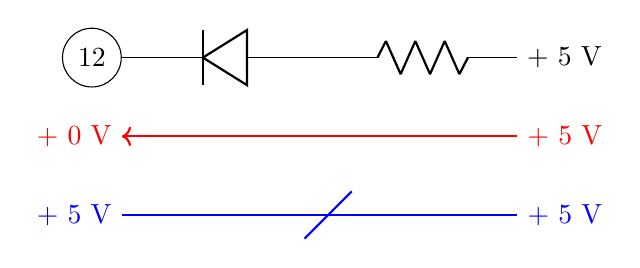
\begin{tikzpicture}
        \node (pin12) [circle, draw=black] at (0,0) {12};
        \node (V5) [] at (6,0) {+ 5 V};

        \draw (V5.west) to[R] (3,0) to[diode] (pin12.east);

        \draw[<-, thick, red] ($(pin12.east) + (0,-1)$) node[anchor=east]{+ 0 V} -- ($(V5.west) + (0,-1)$) node[anchor=west]{+ 5 V};
        \draw[thick, blue] ($(pin12.east) + (0,-2)$) node[anchor=east]{+ 5 V} -- ($(V5.west) + (0,-2)$) node[anchor=west]{+ 5 V};
        \draw[thick, blue] ($(3,-2) - (0.3,0.3)$) -- ($(3,-2) + (0.3,0.3)$);
    \end{tikzpicture}
\end{center}










\subsection{Résolution de l'exercice}





\begin{lstlisting}[frame=single]
#define LED 12
#define PIN 2

void setup()
{
    pinMode(LED, OUTPUT);
    pinMode(PIN, INPUT_PULLUP);
}

void loop()
{
    bool mode = digitalRead(PIN);
    digitalWrite(LED, mode);
}
\end{lstlisting}

On utilise une résistance de 250 $ \Omega $.
\begin{center}
    \includegraphics[width=0.85\textwidth]{images/labo1-manip2.PNG}
\end{center}










\section{Télérupteur}





Explication du code:
\begin{itemize}
    \item On veut changer l'état de la led quand on relache le bouton.
    \item Quand le bouton est pressé, l'état est \textit{LOW} parce qu'on est connecté à la masse.
    \item Et quand on relache, l'état est \textit{HIGH} (à cause de input\_pullup).
\end{itemize}

\begin{lstlisting}[frame=single]
#define LED 12
#define PIN 2

void setup()
{
    pinMode(LED, OUTPUT);
    pinMode(PIN, INPUT_PULLUP);
}

bool etat_precedant = HIGH; // INPUT_PULLUP ==> HIGH
bool etat_led = LOW;

void loop()
{
    bool etat = digitalRead(PIN);
    
    // si on vient de relacher le bouton
    if (etat == HIGH && etat_precedant == LOW)
    {
        // on inverse l'etat de la led
        etat_led = !etat_led;
    }
    
    digitalWrite(LED, etat_led);
    etat_precedant = etat;
}
\end{lstlisting}

On utilise une résistance de 250 $ \Omega $.

\begin{center}
    \includegraphics[width=0.85\textwidth]{images/labo1-manip3.PNG}
\end{center}










\section{Mesure analogique et PWM}





Explication du code : il faut mettre le pin 11 pour la led parce que le 12 n'avait pas de $ \sim $ et ne peut donc pas gérer la fonction \textit{analogWrite}.

\begin{lstlisting}[frame=single]
#define LED 11
#define PIN 2
#define POT A0

void setup()
{
    pinMode(LED, OUTPUT);
    pinMode(PIN, INPUT_PULLUP);
    pinMode(POT, INPUT);
}

bool etat_precedant = HIGH; // INPUT_PULLUP ==> HIGH
bool etat_led = HIGH;

void loop()
{
    bool etat = digitalRead(PIN);
    int val_pot = analogRead(POT);           // 0 a 1023
    //val_pot = map(val_pot, 0,1023, 0,255); // 0 a 255
    val_pot = map(val_pot, 0,1023, 255,0);   // 255 a 0

    // si on vient de relacher le bouton
    if (etat == HIGH && etat_precedant == LOW)
    {
        // on inverse l'etat de la led
        etat_led = !etat_led;
    }
    
    if (etat_led == HIGH)
    {
        analogWrite(LED, val_pot);
    }
    
    etat_precedant = etat;
}
\end{lstlisting}

\begin{center}
    \includegraphics[width=0.85\textwidth]{images/labo1-manip4.PNG}
\end{center}










\section{Clignotement Led}





\begin{lstlisting}[frame=single]
#define LED 8

void setup()
{
    pinMode(LED, OUTPUT);
}

void loop()
{
    digitalWrite(LED, HIGH);
    delay(1000); // Attendre 1000 millisecond (= 1s)
    digitalWrite(LED, LOW);
    delay(1000);
}
\end{lstlisting}

On utilise une résistance de 250 $ \Omega $.
\begin{center}
    \includegraphics[width=0.85\textwidth]{images/labo1-manip6.PNG}
\end{center}










\section{Détection de lumière et hystérésis}










\subsection{Photorésistance}





Pour connaître la résistance de la photorésistance dans tinkercad, on place la photorésistance et un multimètre configuré en ohmmètre et on mesure la variation de la résistance quand on change la luminosité.
\begin{center}
    \includegraphics[width=0.85\textwidth]{images/VoltmetreTinkerCAD.PNG}
\end{center}
Variation de la résistance:
\begin{itemize}
    \item dans le noir = 180 $ k\Omega $,
    \item à la lumière = 506 $ \Omega $.
\end{itemize}










\subsection{Pont diviseur}





\begin{center}
    \includegraphics[width=0.4\textwidth]{images/pont-diviseur-tension.png}
    \hspace{1cm}
    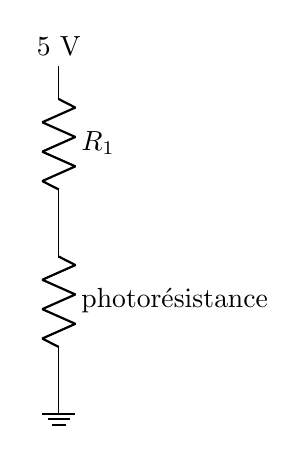
\begin{tikzpicture}
        \draw (0,0) to[R=photorésistance] (0,-2) node[ground]{};
        \draw (0,2) node[anchor=south]{5 V} to[R=$R_1$] (0,0);
    \end{tikzpicture}
\end{center}
Formule pour le calcul de $ R_1 $:
\[ \begin{aligned}
    R_1
    &= \sqrt{\frac{R_{2,min} \times R_{2,max}^2 - R_{2,max} \times R_{2,min}^2}{R_{2,max} - R_{2,min}}} \\
    &= \sqrt{\frac{506 \times (180k)^2 - 180k \times 506^2}{180k - 506}} \\
    &= 9543.58 \; \Omega
\end{aligned} \]
\begin{center}
    \includegraphics[width=0.85\textwidth]{images/pont-diviseur-2.PNG}
\end{center}
Avec une résistance de 9543,58 $ \Omega $:
\begin{itemize}
    \item Tension dans le noir: 4,80 V.
    \item Tension à la lumière: 321 mV.
\end{itemize}
Avec une résistance de 10 $ k\Omega $:
\begin{itemize}
    \item Tension dans le noir: 4,74 V.
    \item Tension à la lumière: 241 mV.
\end{itemize}










\subsection{Pourcentage de lumière}





\begin{center}
    \includegraphics[width=0.75\textwidth]{images/pourcentage-lumiere-1.PNG}
\end{center}





Nous devons mesurer la tension et la convertir en pourcentage de la lumière mesurée. On le fait en 2 étapes:
\begin{enumerate}

\item Mesurer les tensions:
\begin{lstlisting}[frame=single]
#define PIN A2

void setup()
{
    pinMode(PIN, INPUT);
        Serial.begin(9600);
}

void loop()
{
    int value = analogRead(PIN);
    Serial.println(value);
}
\end{lstlisting}
Valeurs mesurées:
\begin{itemize}
    \item dans le noir: 969,
    \item à la lumière: 49.
\end{itemize}

\item Convertir les tensions en pourcentage:
\begin{lstlisting}[frame=single]
#define PIN A2

void setup()
{
    pinMode(PIN, INPUT);
    Serial.begin(9600);
}

void loop()
{
    int value = analogRead(PIN);
    Serial.println( map(value, 969,49, 0,100) );
}
\end{lstlisting}

\end{enumerate}










\subsection{Hystérésis}






\begin{center}
    \includegraphics[width=0.75\textwidth]{images/hysteresis-1.png}
\end{center}
Dans ce cas-ci, nous devons éteindre la LED progressivement en fonction de la luminosité:
\begin{itemize}
    \item luminosité > 90 \% $ \implies $ LED éteinte,
    \item luminosité < 90 \% $ \implies $ LED allumée.
\end{itemize}
Voici 2 solutions:
\begin{itemize}
\item Version 1, LED connectée au 5 V:
\begin{center}
    \includegraphics[width=0.75\textwidth]{images/hysteresis-2.PNG}
\end{center}
\begin{lstlisting}[frame=single]
#define PIN A2
#define LED 3

void setup()
{
    pinMode(PIN, INPUT);
    pinMode(LED, OUTPUT);
    Serial.begin(9600);
}

void loop()
{
    char luminosite = map(analogRead(PIN), 49,968, 100,0);

    if (luminosite >= 93)
        digitalWrite(LED, HIGH); // eteint la led
    if (luminosite <= 87)
        analogWrite(LED, map(luminosite, 0,100, 0,255));
}
\end{lstlisting}
\item Version 2, LED connectée à la masse:
\begin{center}
    \includegraphics[width=0.75\textwidth]{images/hysteresis-3.PNG}
\end{center}
\begin{lstlisting}[frame=single]
#define PIN A2
#define LED 3

void setup()
{
    pinMode(PIN, INPUT);
    pinMode(LED, OUTPUT);
    Serial.begin(9600);
}

void loop()
{
    char luminosite = map(analogRead(PIN), 49,968, 100,0);

    if (luminosite >= 93)
        digitalWrite(LED, LOW); // eteint la led
    if (luminosite <= 87)
        analogWrite(LED, map(luminosite, 0,100, 255,0));
}    
\end{lstlisting}
\end{itemize}

















\section{Alimentation de plusieurs LED en série}





\begin{enumerate}
    \item Schéma 1:
    \begin{center}
        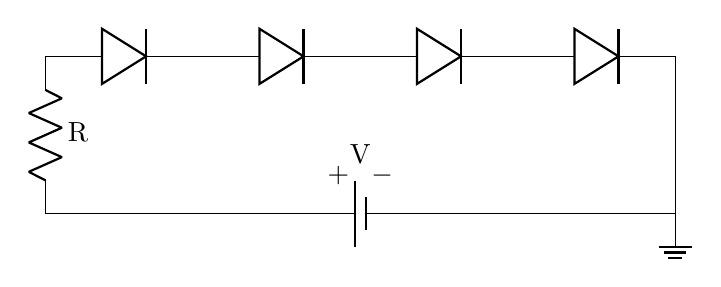
\begin{tikzpicture}
            \draw (0,0) to[diode] (2,0) to[diode] (4,0) to[diode] (6,0) to[diode] (8,0);
            \draw (0,0) to[R=R] (0,-2) to [battery1=V] (8,-2) node[ground]{} -- (8,0);
        \end{tikzpicture}
    \end{center}
    Ce premier schéma est impossible à réaliser en mettant un arduino comme source de courant (à la place de V) car il faudrait supporter 2 V par diode (donc 8 V en tout) et l'arduino ne peut fournir que 5 V au maximum.
    \item Schéma 2:
    \begin{center}
        \begin{tikzpicture}
            \node (npn) [npn] at (0,-5) {};
            \draw (0,0) to[diode] (0,-1) to[diode] (0,-2) to[diode] (0,-3) to[diode] (0,-4) -- ($(npn.C)$);
            \draw (npn.E) -- (0,-8) node[]{\textbullet};
            \draw (0,0) to[R=$R_c$] (3.5,0) to[battery1=batterie] (3.5,-8) -- (0,-8) node[ground]{};
            \draw (npn.B) to[R=$R_b$] ($(npn.B) + (-2,0)$) to[battery1=arduino] ($(npn.B) + (-2,-3)$) -- (0,-8);
        \end{tikzpicture}
    \end{center}
\end{enumerate}
On connaît les valeurs suivantes:
\begin{itemize}
    \item $ I_c $ = 20 mA, pour passer dans les diodes,
    \item $ V_{batterie} $ = 9 V, c'est la seule batterie dans tinkercad,
    \item $ \beta_{cc} $ = 292, donné dans l'énoncé,
    \item $ V_{arduino} $ = 5 V,
    \item $ V_{diode} $ = 2 V,
    \item $ V_{transistor} $ = 0,3 V = différence de tension entre le collecteur et l'émetteur,
    \item $ V_{diode/transistor} $ = 0,7 V = différence de tension entre la base et l'émetteur.
\end{itemize}
On utilise la loi des mailles (maille de droite) pour calculer $ R_c $:
\[ V_{batterie} - R_c \times I_c - 4 \times V_{diode} - V_{transistor} = 0 \]
\[
    \implies R_c
    = \frac{V_{batterie} - 4 \times V_{diode} - V_{transistor}}{I_c}
    = 35 \; \Omega
\]
On calcule $ I_b $ avec:
\[
    I_c = \beta_{cc} \times I_b
    \implies I_b
    = \frac{I_c}{\beta_{cc}}
    = 0,0685 \; \text{mA}
\]
Avec la loi des mailles (maille de gauche), on peut trouver $ R_b $:
\[ V_{arduino} - R_b \times I_b - V_{diode/transistor} = 0 \]
\[
    \implies R_b
    = \frac{V_{arduino} - V_{diode/transistor}}{I_b}
    = 62.8 \; k\Omega
\]





\begin{center}
    \includegraphics[width=0.99\textwidth]{images/leds-serie.PNG}
\end{center}
\textcolor{red}{\textbf{Attention !}} Il faut connecter la masse de l'arduino à la masse de la pile (comme sur le schéma théorique).
\begin{lstlisting}[frame=single]
#define PIN A2
#define LED 3

void setup()
{
    pinMode(PIN, INPUT);
    pinMode(LED, OUTPUT);
}

void loop()
{
    // 49 - 969
    int valLum = analogRead(PIN);

    analogWrite(LED, map(valLum, 49,969, 0,255));
}
\end{lstlisting}





\textbf{Remarque:} si on va voir la datasheet du transistor \textit{BC547} sur le site de \textit{farnell}\footnote{http://www.farnell.com/datasheets/59764.pdf}, on a un $ \beta_{cc,min} = 110 $.















\section{Alimentation de plusieurs LED en parallèle}





\begin{enumerate}
    \item Schéma 1:
    \begin{center}
        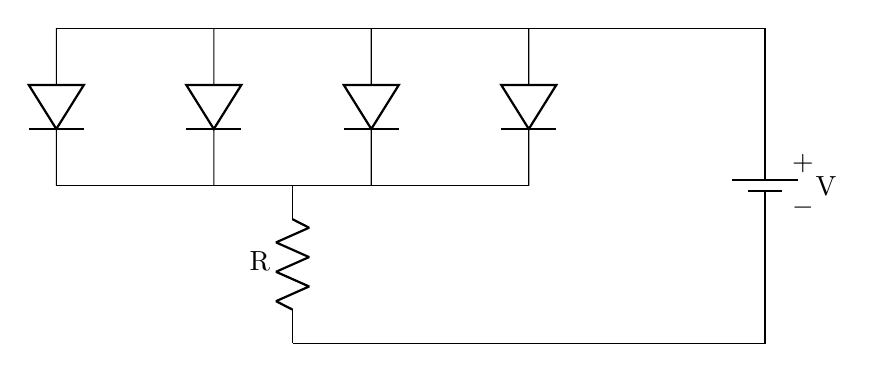
\begin{tikzpicture}
            \draw (0,2) to[R=R] (0,4);

            \draw (-3,6) to[diode] (-3,4);
            \draw (-1,6) to[diode] (-1,4);
            \draw (+1,6) to[diode] (+1,4);
            \draw (+3,6) to[diode] (+3,4);
            \draw (-3,4) -- (3,4);

            \draw (-3,6) -- (6,6) to[battery1=V] (6,2) -- (0,2);
        \end{tikzpicture}
    \end{center}
    Dans ce cas-ci, on n'a pas besoin de pile pour faire ce circuit car on a besoin:
    \begin{itemize}
        \item d'un voltage de 2 V,
        \item d'un courant de $ 4 \times 20 $ mA.
    \end{itemize}
    Et l'arduino peut nous fournir cela à partir de la pin de 5 V (max 200 mA), \textbf{mais} pas depuis une pin I/O normale (max 40 mA). On aura donc besoin d'un transistor.
    \item Schéma 2:
    \begin{center}
        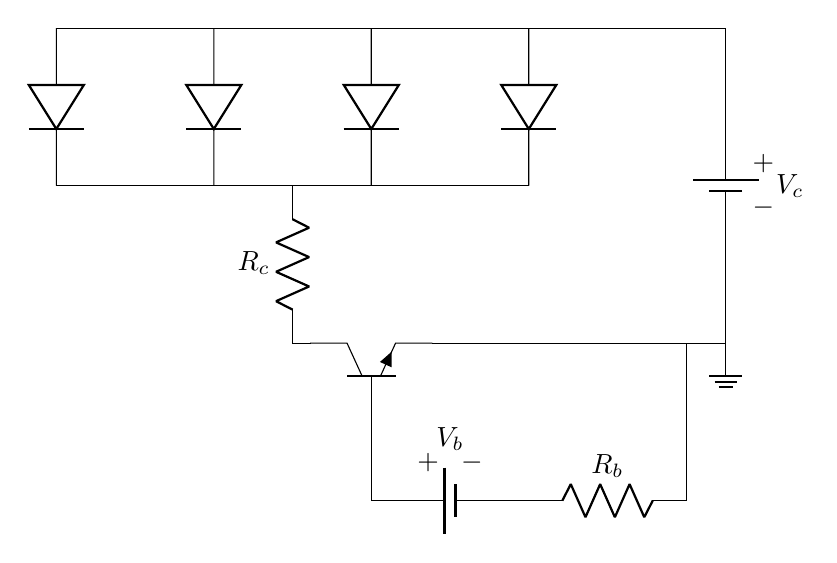
\begin{tikzpicture}
            \draw (-3,6) to[diode] (-3,4);
            \draw (-1,6) to[diode] (-1,4);
            \draw (+1,6) to[diode] (+1,4);
            \draw (+3,6) to[diode] (+3,4);
            \draw (-3,4) -- (3,4);

            \node (npn) [npn, rotate=90] at (1,2) {};

            \draw (npn.C) -- (0,2) to[R=$R_c$] (0,4);
            \draw (-3,6) -- (5.5,6) to[battery1=$V_c$] (5.5,2) node[ground]{} -- (npn.E);
            \draw let \p1 = (npn.B) in ($(npn.B)$) -- (\x1,0) to[battery1=$V_b$] (3,0) to[R=$R_b$] (5,0) -- (5,2);
        \end{tikzpicture}
    \end{center}
\end{enumerate}
On connaît les valeurs suivantes:
\begin{itemize}
    \item $ \beta_{cc} $ = 292, donné dans l'énoncé,
    \item $ I_c $ = 80 mA, pour passer dans les diodes,
    \item $ V_{c} = V_b $ = 5 V,
    \item $ V_{diode} $ = 2 V,
    \item $ V_{transistor} $ = 0,3 V = différence de tension entre le collecteur et l'émetteur,
    \item $ V_{diode/transistor} $ = 0,7 V = différence de tension entre la base et l'émetteur.
\end{itemize}
On utilise la loi des mailles (maille du haut) pour calculer $ R_c $:
\[ V_b - I_c \times R_c - V_{diode} - V_{transistor} = 0 \]
\[
    \implies R_c
    = \frac{V_b - V_{diode} - V_{transistor}}{I_c}
    = 33,75 \; \Omega
\]
On calcule $ I_b $ avec:
\[ I_b = \frac{I_c}{\beta_{cc}} = 0,274 \; mA \]
Avec la loi des mailles (maille du bas) pour calculer $ R_b $:
\[ V_b - I_b \times R_b - V_{diode/transistor} \]
\[
    \implies R_b
    = \frac{V_b - V_{diode/transistor}}{I_b}
    = 15.69 \; k \Omega
\]

\begin{center}
    \includegraphics[width=0.99\textwidth]{images/leds-para.PNG}
\end{center}
\begin{lstlisting}[frame=single]
#define PIN A2
#define LED 3

void setup()
{
    pinMode(PIN, INPUT);
    pinMode(LED, OUTPUT);
    Serial.begin(9600);
}

void loop()
{
    // 49 - 969
    int value = analogRead(PIN);
    Serial.println(value);

    analogWrite(LED, map(value, 49,969, 0,255));
}
\end{lstlisting}















\section{Commande d'un moteur}





\begin{center}
    \begin{tikzpicture}
        \node (npn) [npn] at (0,-5) {};
        \node (motor) [elmech] at (0,-2) {M};
        \draw[thick,->>](motor.right)--++(1,0)node[midway,above]{$\omega$};

        \draw (motor) -- (0,0);
        \draw (motor) -- (npn.C);

        \draw (0,-4) -- (-3,-4) to[diode] (-3,0) -- (0,0);

        \draw (npn.E) -- (0,-8);
        \draw (0,0) -- (3.5,0) to[battery1=batterie] (3.5,-8) -- (0,-8) node[ground]{};
        \draw (npn.B) to[R=$R_b$] ($(npn.B) + (-2,0)$) to[battery1=arduino] ($(npn.B) + (-2,-3)$) -- (0,-8);
    \end{tikzpicture}
\end{center}
On connaît les valeurs suivantes:
\begin{itemize}
    \item $ \beta_{cc} $ = 292
    \item $ V_{arduino} $ = 5 V
    \item $ V_{transistor/diode} $ = 0,7 V
\end{itemize}
Mesure du courant qui sort de la pile pour passer dans le moteur:
\begin{center}
    \includegraphics[width=0.85\textwidth]{images/mesure-courant-pile.PNG}
\end{center}
On a donc: $ I_c $ = 140 mA. On peut calculer:
\[
    R_b
    = \frac{V_{arduino} - V_{transistor/diode}}{I_c / \beta_{cc}}
    = 8968.57 \; \Omega
\]





\begin{center}
    \includegraphics[width=0.99\textwidth]{images/commande-moteur-1.PNG}
\end{center}
\begin{lstlisting}[frame=single]
#define PIN A3
#define MOTEUR 3

void setup()
{
    pinMode(PIN, INPUT);
    pinMode(MOTEUR, OUTPUT);
    Serial.begin(9600);
}

void loop()
{
    // 0 - 1023
    int value = analogRead(PIN);
    Serial.println(value);

    analogWrite(MOTEUR, map(value, 0,1023, 0,255));
}    
\end{lstlisting}




















\newpage \appendix




















\section{Code couleur des résistances}





Jusqu'ici, on a utilisé que des résistances de 250, 1k et 10k $ \Omega $, voici les couleurs pour les identifier:
\begin{itemize}
    \item 250 $ \Omega $ = rouge + vert + marron
    \item 1k $ \Omega $ = marron + noir + rouge
    \item 10k $ \Omega $ = marron + noir + orange
\end{itemize}

\begin{center}
    \includegraphics[width=0.65\textwidth]{images/couleur-resistance.jpg}
\end{center}















\section{Transistor}





\begin{center}
    \begin{tikzpicture}
        \node (N1) [rect, minimum width=1cm] at (0,1) {N};
        \node (P) [rect, minimum width=1cm] at (0,0) {P};
        \node (N) [rect, minimum width=1cm] at (0,-1) {N};

        \draw (0.5,-2.5) node[]{\textbullet} -- (N);
        \draw (0.5,1.5) node[]{\textbullet} -- (N1);
        \draw (-0.5,-0.5) node[]{\textbullet} -- (P);

        \node [anchor=east, red, xshift=-0.2cm] at (-0.5,-0.5) {B};
        \node [anchor=south, yshift=0.2cm] at (0.5,1.5) {C};
        \node [anchor=north, red, yshift=-0.2cm] at (0.5,-2.5) {E};

        \node (npn) [npn, anchor=west] at (2.5,-0.5) {};

        \node [] at (npn.B) {\textbullet};
        \node [] at (npn.C) {\textbullet};
        \node [] at (npn.E) {\textbullet};

        \node [anchor=east, red, xshift=-0.2cm] at (npn.B) {B};
        \node [anchor=south, yshift=0.2cm] at (npn.C) {C};
        \node [anchor=north, red, yshift=-0.2cm] at (npn.E) {E};
    \end{tikzpicture}
    \hspace{4cm}
    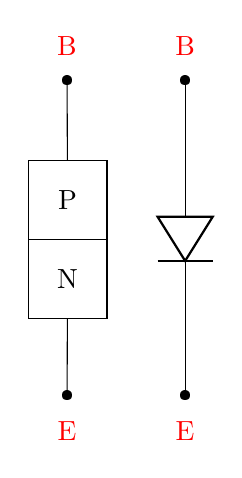
\begin{tikzpicture}
        \node (P) [rect, minimum width=1cm] at (0,0) {P};
        \node (N) [rect, minimum width=1cm] at (0,-1) {N};

        \draw (0.5,1) node[]{\textbullet} -- (P);
        \draw (0.5,-3) node[]{\textbullet} -- (N);

        \draw (2,1) node[]{\textbullet} to[diode] (2,-3) node[]{\textbullet};

        \node [anchor=south, red, yshift=0.2cm] at (0.5,1) {B};
        \node [anchor=north, red, yshift=-0.2cm] at (0.5,-3) {E};
        \node [anchor=south, red, yshift=0.2cm] at (2,1) {B};
        \node [anchor=north, red, yshift=-0.2cm] at (2,-3) {E};
    \end{tikzpicture}
\end{center}
\begin{center}
    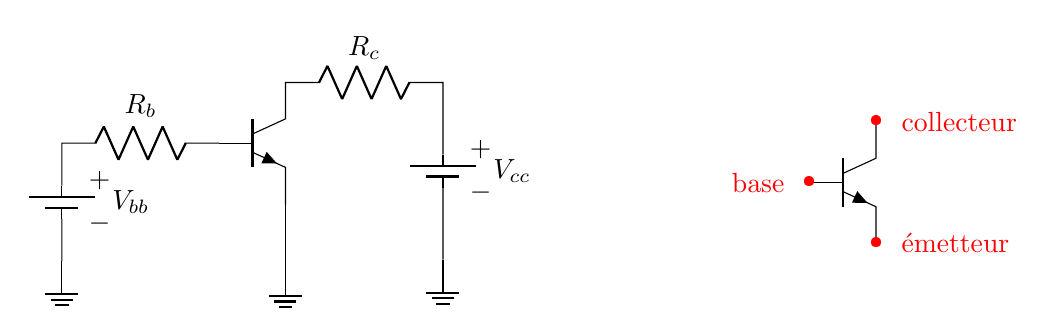
\begin{tikzpicture}
        \node (npn) [npn] at (-4,-0.5) {};

        \draw (npn.C)
            to[R=$R_c$] ($(npn.C) + (2,0)$)
            to[battery1=$V_{cc}$] ($(npn.C) + (2,-2.25)$) node[ground]{};
        \draw (npn.E) -- ($(npn.E) + (0,-0.75)$) node[ground]{};
        \draw (npn.B)
            to[R] ($(npn.B) + (-2,0)$)
            to[battery1=$V_{bb}$] ($(npn.B) + (-2,-1.5)$) node[ground]{};
        \node [anchor=south] at ($(npn.B) + (-1,0.2)$) {$R_b$};


        \node (npn) [npn] at (3.5,-1) {};

        \node [red] at (npn.B) {\textbullet};
        \node [red] at (npn.C) {\textbullet};
        \node [red] at (npn.E) {\textbullet};

        \node [anchor=east, red, xshift=-0.2cm] at (npn.B) {base};
        \node [anchor=west, red, xshift=0.2cm] at (npn.C) {collecteur};
        \node [anchor=west, red, xshift=0.2cm] at (npn.E) {émetteur};
    \end{tikzpicture}
\end{center}

Si: $\displaystyle \beta_{cc} \times I_b < \frac{V_{cc} - 0,3}{R_c} $, alors:
\begin{itemize}
    \item $\displaystyle I_c = \beta_{cc} \times I_b =  \frac{V_{cc} - 0,3}{R_c} $
    \item $\displaystyle I_b = \frac{V_{bb} - 0,7}{R_b} $
\end{itemize}
(équations données dans le cours, probablement basée sur la loi des mailles)

\begin{center}
    \includegraphics[width=0.35\textwidth]{images/transistor.PNG}
\end{center}

\textbf{Remarque:} le transistor dans tinkercad est le BC546.















\section{Caractéristiques de l'arduino}





\begin{itemize}
    \item Courant max pour les pins \textbf{GND} et \textbf{5V} = 200 mA.
    \item Courant max pour les autres pins = 40 mA.
    \item Voltage max pour toutes les pins = 5 V.
    \item Voltage min pour toutes les pins = 0 V.
\end{itemize}















\section{Caractéristiques des LED vertes}





\begin{itemize}
    \item Courant max = 20 mA.
    \item Voltage max = 2 V.
\end{itemize}















\section{Mesure du $ \beta_{cc} $ dans tinkercad}





\begin{center}
    \includegraphics[width=0.99\textwidth]{images/calcul-beta-cc.PNG}
\end{center}

On vient de mesurer $ I_c $ = 62,3 mA et $ I_b $ = 213 $ \mu $A. On peut donc calculer $ \beta_{cc} $:
\[ \beta_{cc} = \frac{I_c}{I_b} = \frac{62,3}{0,213} \approx 292,5 \]















\newpage \section{Méthode examen}





\begin{enumerate}


\item Choisir si on fait un circuit en parallèle ou en série et la source d'alimentation principale
\begin{example}
    Caractéristiques des composants :
    \begin{itemize}
        \item led (max) : 2.12 V, 20 mA
        \item pin arduino : 5 V, ($I_{max}$) 40 mA
        \item 5V/masse arduino : 5 V, ($I_{max}$) 200 mA
        \item pile : 9 V
    \end{itemize}
\end{example}


\item Faire un dessin du circuit sans le transistor
\begin{example}
    Seulement :
    \begin{itemize}
        \item la source de tension
        \item les leds
    \end{itemize}
\end{example}


\item Ajouter le transistor sur le dessin (si nécessaire)
\begin{example}
    Remarques :
    \begin{itemize}
        \item le transistor se trouve \textbf{entre les leds et la masse}
        \item l'émetteur du transistor (E) est connecté à la masse
        \item les leds sont connectées au transistor par le collecteur (C)
        \item la pin qui commande le transistor est connectée à la base (B) avec une résistance entre les 2
    \end{itemize}
\end{example}


\item Ajouter une résistance avant (ou après) les leds et calculer sa valeur
\begin{example}
    \[ R = \frac{V_{source} - V_{led} - 0.3 \; [V]}{I_{led}} \]
\end{example}


\item Ajouter une résistance à la base du transistor et calculer sa valeur
\begin{example}
\[ R = \frac{V_{arduino} - 0.7 \; [V]}{I_b} \]
avec
\[ I_b = \frac{I_c}{\beta_{cc}} = \frac{I_{led}}{\beta_{cc}} \qquad (\beta_{cc} = 292) \]
\end{example}


\item Faire le schéma sur tinkercad
\begin{example}
    Remarques :
    \begin{itemize}
        \item commencer avec le 5V et la masse
        \item si il y a une pile, connecter les masses entre elles
        \item ajouter le transistor, les leds (ctrl+c, ctrl+v pour aller plus vite)
        \item mettre les résistances (attention aux valeurs)
        \item tout connecter avec des câbles
        \item puis, ajouter les boutons, etc.
    \end{itemize}
    Pour le bouton en input\_pullup :
    \begin{center}
        \includegraphics[width=0.4\textwidth]{images/bouton-input-pullup.PNG}
    \end{center}
    Pour le potentiomètre :
    \begin{center}
        \includegraphics[width=0.5\textwidth]{images/potentiometre.PNG}
    \end{center}
    Pour la photorésistance :
    \begin{center}
        \includegraphics[width=0.5\textwidth]{images/photoresistance.PNG}
    \end{center}
\end{example}


\item Faire le code
\begin{enumerate}

    \item On \texttt{define} toutes les pins utilisées
    \begin{example}
        ex : \texttt{\#define LED 7}
    \end{example}

    \item Dans \texttt{void setup()}
    \begin{enumerate}
        \item on donne un mode pour chaque pin utilisée
        \begin{example}
            ex :
            \begin{itemize}
                \item \texttt{pinMode(LED, INPUT);}
                \item \texttt{pinMode(BUT, INPUT\_PULLUP);}
                \item \texttt{pinMode(BUT, OUTPUT);}
            \end{itemize}
        \end{example}
        \item on fait : \texttt{Serial.begin(9600);}
    \end{enumerate}

    \item Dans \texttt{void loop()}
    \begin{enumerate}
        \item on lit les valeur sur les pin configurées en input (ou input\_pullup)
        \begin{example}
            ex :
            \begin{itemize}
                \item \texttt{bool mode = digitalRead(PIN);} // 0 à 1
                \item \texttt{int val = analogRead(PIN);} // 0 à 1023
                \item \texttt{unsigned int val = analogRead(PIN);} // 0 à 1023
            \end{itemize}
        \end{example}
        \item afficher les valeurs lues (si nécessaire)
        \begin{example}
            ex : \texttt{Serial.println(value);}
        \end{example}
        \item Convertir ces valeurs (si nécessaire)
        \begin{example}
            ex :
            \begin{itemize}
                \item \texttt{char percent = map(value, 0,1023, 0,100)} // value (0-1023), percent (0-100)
                \item \texttt{char percent = map(value, 0,1023, 100,0)} // value (0-1023), percent (100-0)
            \end{itemize}
        \end{example}
        \item écrire les conditions et renvoyer des valeurs sur les outputs
        \begin{example}
            ex : \texttt{if (val > 90) \{ digitalWrite(LED, HIGH); \}}
        \end{example}
    \end{enumerate}

    \item Si il faut un bouton télérupteur
    \begin{enumerate}
        \item on define la pin utilisée
\begin{lstlisting}[frame=single]
#define BTN 3
\end{lstlisting}
        \item dant setup, on met la pin en mode INPUT\_PULLUP
\begin{lstlisting}[frame=single]
pinMode(BTN, INPUT_PULLUP);
\end{lstlisting}
\item on définit (en-dehors de setup et loop) :
\begin{lstlisting}[frame=single]
bool etat_precedant_BTN = HIGH; // INPUT_PULLUP ==> HIGH
bool etat_led = LOW;
\end{lstlisting}
        \item dans loop,
\begin{lstlisting}[frame=single]
bool etat_BTN = digitalRead(BTN);
// si on vient de relacher le bouton
if (etat_BTN == HIGH && etat_precedant_BTN == LOW) {
    etat_led = !etat_led; // on inverse l'etat de la led
}
digitalWrite(LED, etat_led);
etat_precedant = etat;
\end{lstlisting}
    \end{enumerate}

\end{enumerate}


\end{enumerate}




















\tableofcontents




















\end{document}
